\documentclass{article}
\usepackage[letterpaper, top=1in, bottom=1in, left=1in, right=1in]{geometry}
\usepackage[utf8]{inputenc}


  \usepackage[english]{babel}
  \usepackage{tikz-cd, extarrows, esvect, esint, pgfplots, lipsum, bm, dcolumn}
  \usetikzlibrary{arrows}
  \usepackage{amsmath, amssymb, amsthm, mathrsfs, mathtools, centernot, hyperref, fancyhdr, lastpage}
  \usepackage{tikz}
  \pgfplotsset{compat=1.18}


  \setlength{\parindent}{0pt} % set no indent
  \hfuzz=5.002pt % ignore overfull hbox badness warnings below this limit


\newtheorem{theorem}{Theorem}[section]
\newtheorem{proposition}[theorem]{Proposition}
\newtheorem{lemma}[theorem]{Lemma}
\theoremstyle{definition}
\newtheorem{example}{Example}[section]
\newtheorem{exercise}{Exercise}[section]
\newtheorem{corollary}{Corollary}[theorem]
\theoremstyle{remark}
\newtheorem*{remark}{Remark}
\theoremstyle{definition}
\newtheorem{definition}{Definition}[section]
\renewcommand{\qed}{\hfill$\blacksquare$}
\renewcommand{\footrulewidth}{0.4pt}% default is 0pt

\newenvironment{solution}{\noindent \textit{Solution.}}{}

\renewcommand{\thispagestyle}[1]{}

\begin{document}
\pagestyle{fancy}

\lhead{CS201}
\chead{Muchang Bahng}
\rhead{\date{Spring 2023}}
\cfoot{\thepage / \pageref{LastPage}}

\title{Data Structures and Algorithms (w/ Java)}
\author{Muchang Bahng}
\date{Spring 2023}

\maketitle

\noindent When a program is build and run, we must worry about two computational overheads: 
\begin{enumerate}
    \item the runtime of the program, which is determined by the efficiency of the algorithm itself 
    \item the memory overhead of the program, which is determined by the types of data structures used. 
\end{enumerate}
When we want to optimize these programs, we therefore want to look at their data structures and algorithms. 

Note that Java has the following \textbf{primitive types}: \texttt{int}, \texttt{long}, \texttt{float}, \texttt{double}, \texttt{boolean}, \texttt{char}. Everything else is a \textbf{reference type}. 

\subsection{References and Memory Allocation}

We can think of our RAM as storing our memory. Whenever we call the  $\texttt{new}$ keyword, we allocate new memory for whatever object we are storing. Say that an $\texttt{int}$ stores $4$ bytes each, and we create an array of ten integers. 
\begin{verbatim}
int[] numbers = new int[10]; 
\end{verbatim}
\begin{center}
    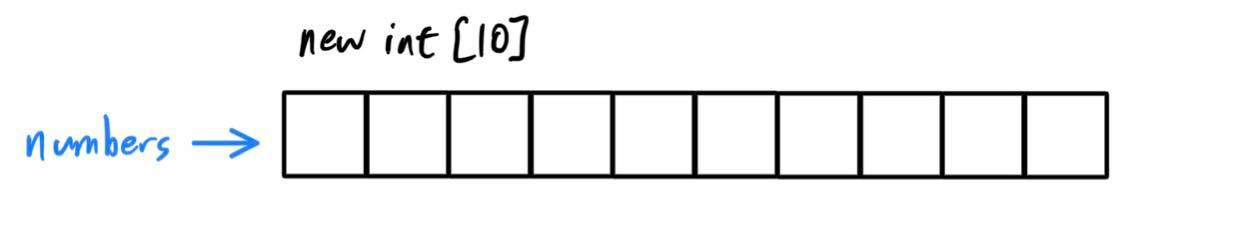
\includegraphics[scale=0.3]{img/reference1.jpg}
\end{center}
This array would take up 40 bytes of memory, and to access this part of the memory, we create a variable $\texttt{numbers}$ that really just stores the location of the object in memory. Since variables are just references to memory locations, we can have multiple variables referencing the same object. Note that we did not use the $\texttt{new}$ keyword here. 
\begin{verbatim}
int[] stuff = numbers; 
\end{verbatim}
\begin{center}
    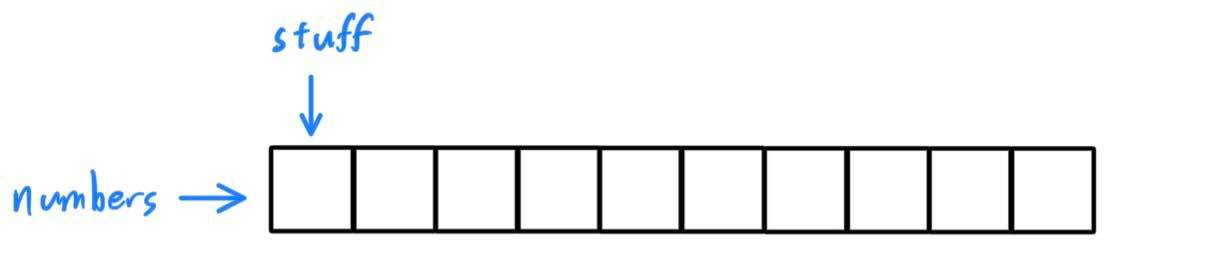
\includegraphics[scale=0.3]{img/reference2.jpg}
\end{center}
Therefore, both $\texttt{numbers}$ and $\texttt{stuff}$ points to the same array, and whatever we do with one is done to the other. If we wanted to create two distinct arrays in memory, we can do this: 
\begin{verbatim}
int[] numbers = new int[10]; 
int[] stuff = new int[10]; 
\end{verbatim}
\begin{center}
    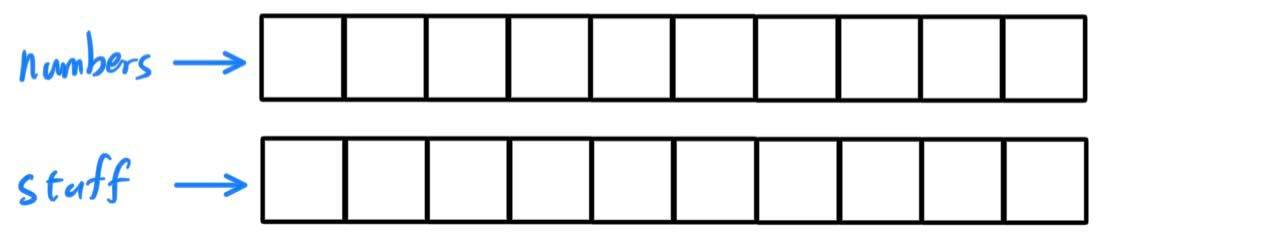
\includegraphics[scale=0.3]{img/reference3.jpg}
\end{center}
which would take up 80 bytes of memory. Therefore, we must distinguish the \textit{actual object in memory} and the \textit{variable that references the object}. Say that the variable is $\texttt{myList}$ and the object that it references to is $\texttt{ArrayList<String> Object}$. Then, we will denote it shorthand as 
\[\texttt{myList} \mapsto \texttt{ArrayList<String> Object}\]

This is all simple enough, but it gets a bit more confusing when we talk about how functions act. When we have some function $\texttt{func}$ and input variable, say $\texttt{myList} \mapsto \texttt{ArrayList<String> Object}$, the function create a \textit{copy of the reference} in the backend, also named $\texttt{myList}$ (confusingly) and acts on this copy. Note now that we are working with two references. 
\begin{center}
    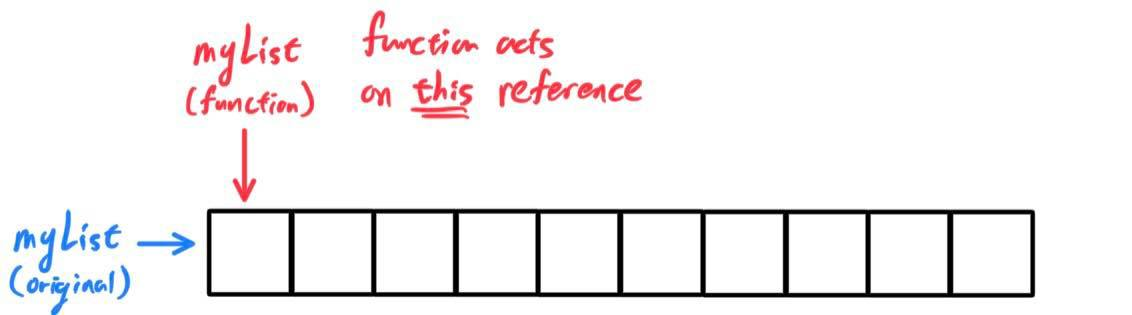
\includegraphics[scale=0.3]{img/functions_on_references.jpg}
\end{center}
Therefore, the function is allowed to modify $\texttt{ArrayList<String> Object}$ through the copied reference variable. 

\begin{example}[Modifying Referred Object]
Given the function 
\begin{verbatim}
public static void removeFront(List<String> words) {
    words.remove(0); // this 'words' is a copy of the reference 
}

List<String> words = new LinkedList<>(); 
words.add("CS"); 
removeFront(words); 
System.out.println(words); // prints [] (empty)
\end{verbatim}
if $\texttt{words}$ references an array of 1 million elements, then $\texttt{removeFront}$ will not copy the entire array and allocate new memory, but it will just act on the original array. 
\begin{center}
    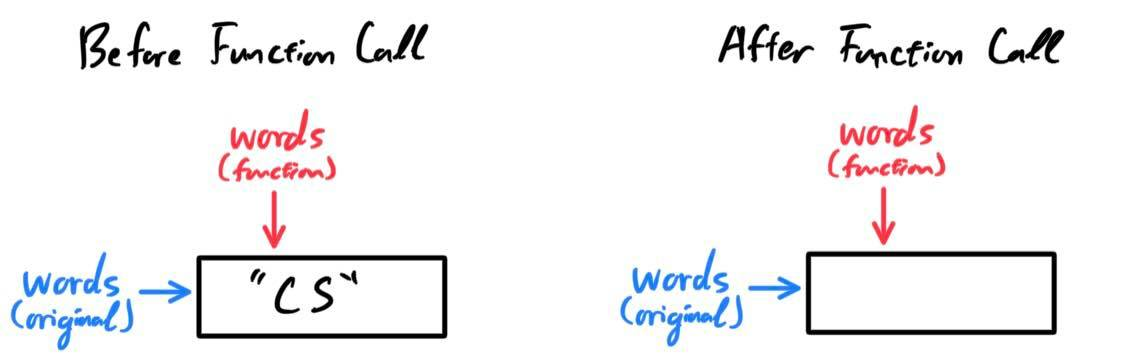
\includegraphics[scale=0.3]{img/func_ref_example1.jpg}
\end{center}
\end{example}

However, it cannot modify the reference of the original variable, and so you cannot "lose" a reference inside a method.  

\begin{example}
Given the function 
\begin{verbatim}
public static void tryBreakReference(List<String> words) {
    words = new LinkedList<>(); // this 'words' is a copy of the reference 
}

List<String> words = new LinkedList<>(); 
words.add("CS"); 
tryBreakReference(words); 
System.out.println(words); // Still prints ["CS"]
\end{verbatim}
This does not affect the object that the original $\texttt{words}$ is referencing to since the function takes only the \textit{copied reference variable} and changes its reference to the new LinkedList. 
\begin{center}
    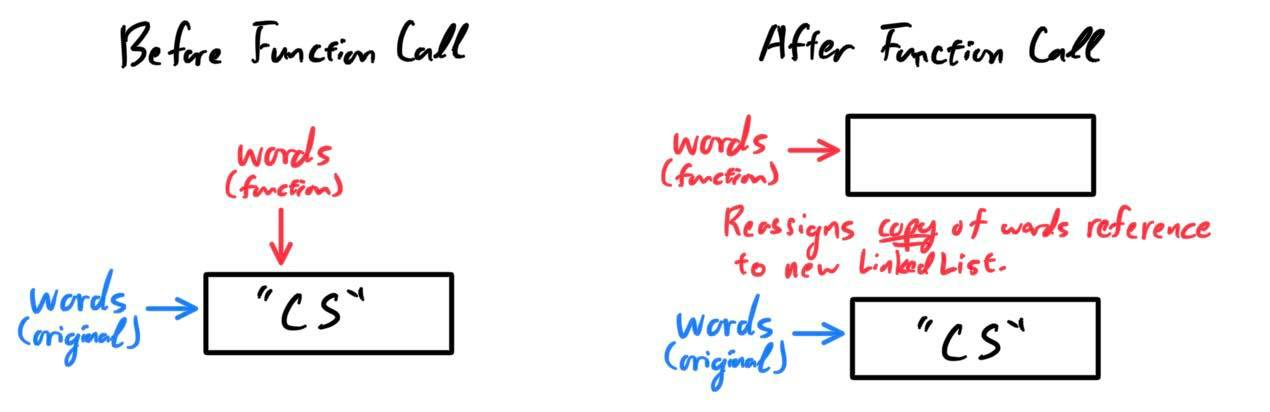
\includegraphics[scale=0.3]{img/func_ref_example2.jpg}
\end{center}
\end{example}

The default value for an uninitialized (no memory allocated by call to $\texttt{new}$) object is $\texttt{null}$. If you try to call any methods to a null object, you will get a \textbf{null pointer exception error}. 

\begin{example}
Let's go through an exercise. Given the code 
\begin{verbatim}
public static ListNode foo(ListNode list) {
    list = list.next; 
    list.next = null; 
    return list; 
}

public static void main(String[] args) {
    ListNode list = new ListNode(2,  new ListNode(0, new ListNode(1))); 
    ListNode ret  = foo(list); 
    printList(ret);     // prints 0 
    printList(list);    // prints 2, 0 
}
\end{verbatim}
Let us examine the behavior of it. Note that we allocate memory for $\texttt{list}$, which we will denote by the reference $\texttt{list}_m$ and when we input it into $\texttt{foo}$, we get a copy of the reference, denoted $\texttt{list}_c$. 
\begin{center}
    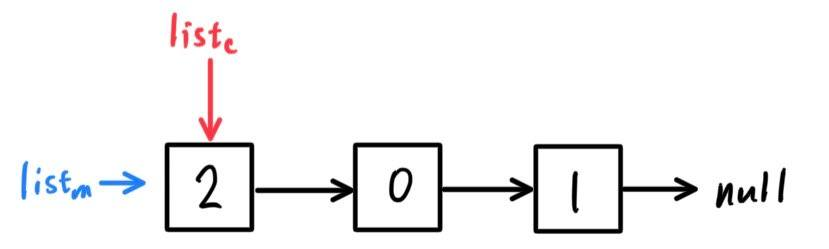
\includegraphics[scale=0.3]{img/step1.jpg}
\end{center}
$\texttt{foo}$ takes $\texttt{list}_c$ and has it reference the next value, which is $0$. Therefore, $\texttt{list}_m$ is $2, 0, 1$ and $\texttt{list}_c$ is $0, 1$. 
\begin{center}
    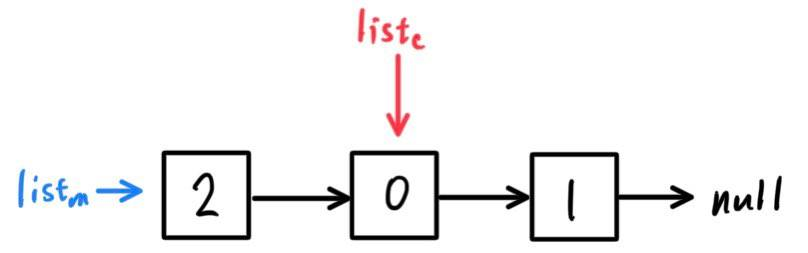
\includegraphics[scale=0.3]{img/step2.jpg}
\end{center}
Now, we set the next value of $\texttt{list}_c$ to null, and since this modifies the LinkedList object, we have both $\texttt{list}_m$ is $2, 0$ and $\texttt{list}_c$ is $0$. 
\begin{center}
    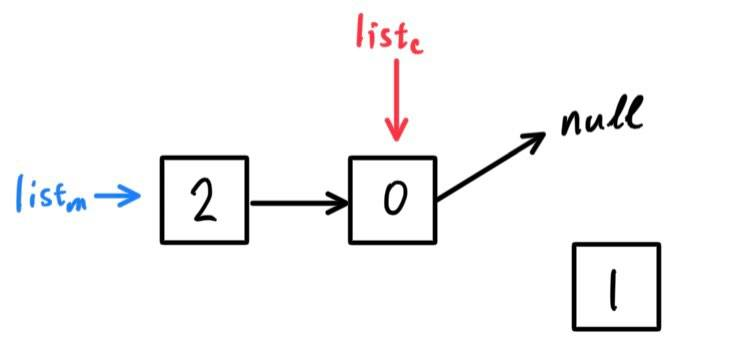
\includegraphics[scale=0.3]{img/step3.jpg}
\end{center}
\end{example}


\subsection{Arrays}

Let us take a look at the most basic data structure in Java: the array. They are mutable, homogeneous (can only store one type), and fixed in size. We can print their outputs by converting them to a string, as such with the static method: 
\begin{verbatim}
System.out.println(Arrays.toString(arr)); 
\end{verbatim}

\subsection{Classes and Objects}

Just like in other object oriented languages, Java uses classes, and everything must be used in a class. Here, we have a class with static and dynamic variables, static and dynamic methods, and constructors. 
\begin{verbatim}
public class Point {
  public static String creator = "Muchang"; // static variable 

  public int x; // dynamic variable
  public int y; // dynamic variable 

  public Point (int x, int y) { // constructor 
    this.x = x; 
    this.y = y; 
  }

  public Point (Point p) { // constructor
    this.x = p.x; 
    this.y = p.y; 
  }

  public double distanceFrom(Point other) { // dynamic method 
    return Math.sqrt((x - other.x)*(x - other.x) + (y - other.y)*(y - other.y)); 
  }
  
  public static void greet() { // static method 
    System.out.println("I am a point!"); 
  }
}
\end{verbatim}

\subsubsection{Public vs Private Variables and Attributes}
Note that every single variable and method had the $\texttt{public}$ keyword, which allows users to read/modify the variables and run the methods, \textit{even outside the class it is defined in}. If we switched them to $\texttt{private}$, then we could still access them within the code, but we would not be able to read/modify them elsewhere. This is particularly useful for when we are dealing with sensitive information, and if we do want to grant users the power to read/modify them, we can use separate public getter and setter methods. 
\begin{verbatim}
public class Point {
  private String name; 
  public int x; 
  private int y;  

  public Point (String name, int x, int y) {
    this.name = name; 
    this.x = x; 
    this.y = y; 
  }
  
  public getName() {    // getter method 
    return this.name; 
  }
  
  public setName(String newName) {  // setter method 
    this.name = newName; 
  }

  private void increment() {
    this.x ++; 
    this.y ++; 
  }

  public static void main(String[] args) {
    Point p = new Point(1, 2); 
    System.out.println(p.x); 
    System.out.println(p.y); // still accessible since within the class 
    p.increment(); // still runnable since within the class 
    System.out.println(p.x); 
    System.out.println(p.y);
  }
}
\end{verbatim}

\subsubsection{Inheritance}

\subsubsection{.equals() method}

Generally for objects, we should use the $\texttt{.equals()}$ method. It must be implemented for the given class. If it is not implemented, then the $\texttt{.equals()}$ just checks memory locations, and so calling $\texttt{p = new Point(0.0, 0.0)}$ and $\texttt{q = new Point(0.0, 0.0)}$ and comparing them with $\texttt{p.equals(q)}$ would return false. When we also create an array of a certain object, we must create the actual objects in the array by calling new. For example, we don't even create the Point objects in an initialized array. 
\begin{verbatim}
Point[] pointArray = new Point[5];  // creates the array and allocates memory 
System.out.println(pointArray[0].x) // but didn't actually create the points, so error
\end{verbatim}
We could also store the same references to the variables. 
\begin{verbatim}
ArrayList<Point> myPoints = new ArrayList<>(); 
Point p = new Point(2.0, 2.0); 
myPoints.add(p); 
p.x = 3.4; 
myPoints.add(p); 

// This creates the ArrayList of form (p, p), which both reference 
// the same Point object, so both of form (3.4, 2.0), (3.4, 2.0). 
\end{verbatim}
So, we should call new for every Point object. 
\begin{verbatim}
ArrayList<Point> myPoints = new ArrayList<>(); 
for (int i = 0; i < 10; i++) {
    myPoints.add(new Point(0.0, 0.0)); 
}
Point p = new Point(0.0, 0.0); 
System.out.println(pointList.contains(p)); 
\end{verbatim}
The final line can print either true or false: 
\begin{enumerate}
    \item It prints false if there is no .equals() method implemented in the Point class. $\texttt{.contains()}$ uses the $\texttt{.equals()}$ method on every element of the ArrayList by running a for loop, so it will use the default implementation of checking references. 
    \item If $\texttt{.equals()}$ is implemented as before, it will check the values of x and y, so it will print true.
\end{enumerate}

\section{Collections Interface}

\textbf{Interfaces} in Java specify functionality by specifying what methods exist. At almost the top, we have the \textbf{collections} interface, which represents "a group of stuff." It is divided into 3 main subinterfaces: Lists, Sets, and Maps (along with many others), which add more functionality. So, an interface represents the functionality of whatever we will create, while the implementation is the actual concrete class. 


\subsection{List Interface}

We want to define a list that has the following methods given some list $\texttt{lst}$. 
\begin{enumerate}
    \item $\texttt{Object y = lst.get(0)}$ outputs the $0$th element. 
    \item $\texttt{boolean y = lst.contains(elem)}$ checks if $\texttt{elem}$ 
    \item $\texttt{lst.add(Object elem)}$ adds the element to the end of the list. 
    \item $\texttt{lst.remove(Object elem)}$ removes the element. 
    \item $\texttt{lst.size()}$ returns size of the list. 
\end{enumerate}

\begin{definition}[ArrayList]
An ArrayList just implements an array in the backend but with some extra systematic way to dynamically grow. If we add to an array, we either have space and can do it, or we don't and can't. If we add to an ArrayList, we can 
\begin{enumerate}
    \item simply add to the first open position if there's space left, $O(1)$ 
    \item we grow the size of the ArrayList by creating a new larger array, copying everything, and then adding to the first open position. (linear time $O(n)$), since we have to add all the elements to the new array.
\end{enumerate}
Starting with a length $1$ array, if we add $N$ elements one at a time and when full, create a new array that is
\begin{enumerate}
    \item is twice as large (geometric growth: 1, 2, 4, 8, 16, ...). Then, we must copy at sizes 1, 2, 4, 8, ... and the total values copied looks like 
    \[1 + 2 + 4 + \ldots + (N/4) + (N/2) = N - 1\]
    This is what the Java.util.ArrayList implements, and you can see the performance of adding is $O(N)$.
    \item has $1$ more position (arithmetic growth: 1, 2, 3, ...). Then, we must copy at sizes 1, 2, 3, 4, ... and the total values copied looks like
    \[1 + 2 + 3 + \ldots + (N - 1) = N (N - 1)/2\]
    If the arithmetic pattern is adding, say 1,000,000 elements, then we are wasteful of memory. 
\end{enumerate}
This geometric growth is a good tradeoff between performance and memory usage. It never uses more than twice the memory of an array in order to store it. Furthermore, the runtime of a geometric growth pattern is amortized constant time, which means that it is constant when averaged over a long time. This is because the vast majority of these operations are constant time, with a few add operations which require resizing to be longer. But these few ones happen less and less frequently that when averaged over a long period, we can treat it as constant. 
\end{definition}

One thing to note is that while adding to the end of an ArrayList can be efficient, adding to the front is not since it must shift the entire Array, even if there is space left.

\begin{theorem}[ArrayList Runtime Complexity]
The following are true for ArrayList $\texttt{lst}$:  
\begin{enumerate}
    \item Getting and Contains 
    \begin{enumerate}
        \item $\texttt{lst.get(int index)}$ is $O(1)$. 
        \item Getting every element is $O(n)$ 
        \item $\texttt{lst.contains(Object elem)}$ is $O(n)$
    \end{enumerate}
    
    \item Adding 
    \begin{enumerate}
        \item $\texttt{lst.add(Object elem)}$ is amortized $O(1)$. 
        \item $\texttt{lst.add(0, Object elem)}$ is $O(n)$. 
        \item $\texttt{lst.add(int index, Object elem)}$ is on average $O(n)$. 
    \end{enumerate}
    
    \item Removing 
    \begin{enumerate}
        \item $\texttt{lst.remove(0)}$ is $O(n)$ 
        \item $\texttt{lst.remove(int index)}$ is $O(n)$ 
        \item $\texttt{lst.remove(lst.size() - 1)}$ is $O(1)$ 
        \item $\texttt{lst.remove(Object elem)}$ 
    \end{enumerate}
\end{enumerate}
\end{theorem}
\begin{proof}
Listed. 
\begin{enumerate}
    \item Getting the element at index $\texttt{index}$ requires us to just look at the same index in the underlying array, which is $O(1)$. 
    \item We loop through each element of the ArrayList and call $\texttt{.equals(elem)}$ at each step, which results in $O(1)$. 
    \item Since the geometric growth of the ArrayList happens exponentially less frequently, it averages out to be $O(1)$, so amortized. 
    \item Adding at a specific index requires $O(n)$ since we create a new ArrayList and copy over all the elements with the added element.  
    \item Removing an object requires us to shift the indices of the remaining elements by $1$, so this is $O(n)$. 
\end{enumerate}
\end{proof}

\begin{example}[String]
The string type is just an ArrayList of characters. It has the following attributes and methods. Let $\texttt{x = "I love CS201"}$ 
\begin{enumerate}
    \item $\texttt{int y = x.length()}$ outputs the length and is $O(1)$ 
    \item $\texttt{char y = x.charAt(0)}$ outputs a character and is $O(1)$
    \item $\texttt{String y = x.substring(0, 4)}$ 
    \item $\texttt{boolean y = x.equals("I love CS201")}$
    \item $\texttt{String y = x + "!!"}$ 
    \item $\texttt{String[] y = x.split(" ")}$
    \item $\texttt{String y = String.join(" ", words)}$
\end{enumerate}
\end{example}

\begin{definition}[Linked List]
A linked list contains a sequence of nodes that each contain an object for its element and a reference to the next node. More specifically, it can be divided up into 3 parts: 
\begin{enumerate}
    \item The variable which points to the \textit{first} node. This can be confusing since this variable, which represents an \textit{entire list} is just a pointer to the first node. 
    \item A sequence of nodes containing the element and a reference to the next node. 
    \item The final node containing the element and a reference to $\texttt{null}$. 
\end{enumerate}
We can implement these functionalities in the $\texttt{ListNode}$ class, which are used to build a linked list of integers. 
\begin{verbatim}
public class ListNode {
    int info;           // value i.e. element 
    ListNode next;      // reference to next ListNode
    
    ListNode(int x) {
        info = x; 
    }
    ListNode(int x, ListNode node) {
        info = x; 
        next = node; 
    }
}
\end{verbatim}
The following diagram represents a linked list. 
\begin{center}
    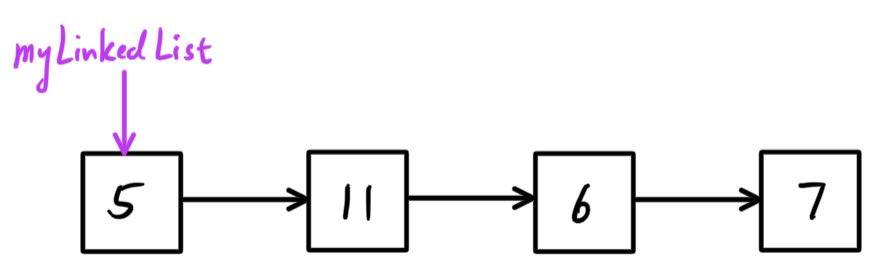
\includegraphics[scale=0.3]{img/linked_list_diagram.jpg}
\end{center}
But in reality, the elements are all located random in memory and can only be found by references. 
\begin{center}
    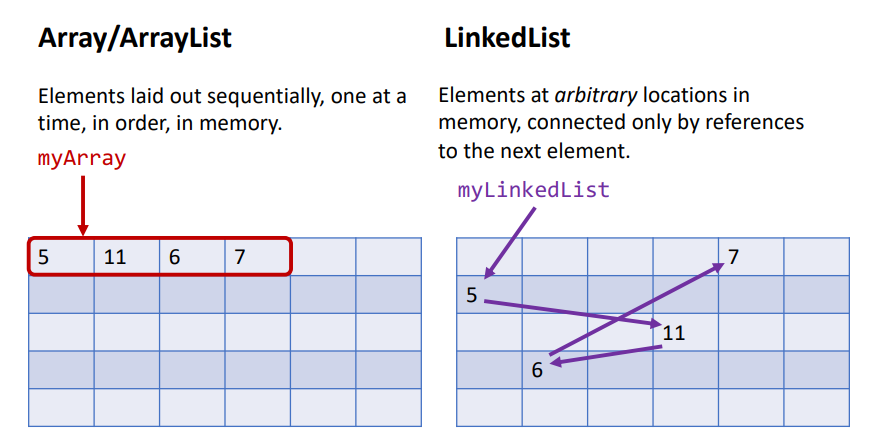
\includegraphics[scale=0.3]{img/linked_list_random_memory.png}
\end{center}
\end{definition}
To print everything in a linked list, we just loop over the nodes as long as the nodes are not null. 
\begin{verbatim}
public static void printList(ListNode list) {
    while (list != null) {          // common conditional for traversing 
        System.out.println(list.info); 
        list = list.next; 
    }
}
\end{verbatim}

\begin{theorem}[Linked List Runtime Complexity]
The following are true for a basic LinkedList $\texttt{lst}$:  
\begin{enumerate}
    \item Getting and contains 
    \begin{enumerate}
        \item $\texttt{lst.get(int index)}$ is $O(n)$ on average (unless you get the first index, which is fast).  
        \item Getting every element in the list is $O(n^2)$. 
        \item $\texttt{lst.contains(Object elem)}$ is $O(n)$ 
    \end{enumerate}
    
    \item Adding 
    \begin{enumerate}
        \item Start:  $\texttt{lst.add(0, Object elem)}$ is $O(1)$ 
        \item Middle: $\texttt{lst.add(int index, Object elem)}$ is on average $O(n)$. 
        \item End:    $\texttt{lst.add(Object elem)}$ is $O(n)$
    \end{enumerate}
    
    \item Removing 
    \begin{enumerate}
        \item Start:  $\texttt{lst.remove(0)}$ or $\texttt{lst.remove()}$ is $O(1)$ 
        \item Middle: $\texttt{lst.remove(int index)}$ is on average $O(n)$ 
        \item End:    $\texttt{lst.remove(lst.size() - 1)}$ is $O(n)$ 
    \end{enumerate}
\end{enumerate}
\end{theorem}
\begin{proof}
Listed. 
\begin{enumerate}
    \item We must traverse from the beginning of the linked list, and so it is $O(n)$. If we just pay attention to the first (or last, for doubly-linked list) element, then this is just $O(1)$. 
    \item Getting every element is just looping an $O(n)$ operation $n$ times, so $O(n^2)$. 
    \item You need to iterate through each element and call $\texttt{.equals(elem)}$, so it is $O(n)$. 
    \item We can simply take the reference 
    \item Adding 
\end{enumerate}
\end{proof}

Even though our basic LinkedList solves the problem of adding in the beginning, in order to add in the middle or end, we must get to that position (which is $O(n)$ time) before we are able to utilize our $O(1)$ add. This is quite inefficient, especially when we do repeated adding, so we should keep track of certain "markers" that indicate where our current node is. \textbf{Iterators} do this naturally, so we would like to implement some current notion of position.Below we implement a new linked list (of integers). 

\begin{definition}[Iterator]
An \textbf{iterator} is a Java interface that has the two methods: 
\begin{enumerate}
    \item $\texttt{.hasnext()}$ checks if there is an element after the current one. 
    \item $\texttt{.next()}$ prints out the next element. 
\end{enumerate}
We want to implement iterators to any collections or whatever custom class if we want to be able to use enhanced for loops over them. 
\end{definition}


\begin{definition}[DIYLinkedList]
Note the following: 
\begin{enumerate}
    \item Adding to the end ($\texttt{add}$) and to the front ($\texttt{addtoFront}$) are both $O(1)$, since we always have access to the dynamic attributes $\texttt{first}$ and $\texttt{last}$. 
\end{enumerate}
\begin{verbatim}
public class DIYLinkedList implements Iterable<Integer> {
    private class ListNode {
        int value; 
        ListNode next; 
        public ListNode(int value) {
            this.value = value; 
        }
        public ListNode(int value, ListNode next) {
            this.value = value; 
            this.next = next; 
        }
    }
    
    private ListNode first; 
    private ListNode last; 
    private int size; 
    
    public DIYLinkedList() {
        size = 0; 
    }
    
    public int size() {
        return size; 
    }
    
    public int get(int index) {
        if (index < 0 || index >= size) {
            throw new IndexOutOfBoundsException(); 
        }
        current = first; 
        for (int i = 0; i < index; i++) {
            current = current.next; 
        }
        return current.value; 
    }
    
    public void add(int elem) { 
        // add to end 
        if (last == null) {
            last = new ListNode(elem); 
            first = last; 
        }
        else {
            last.next = new ListNode(elem); 
            last = last.next; 
        }
        size++; 
    }
    
    public void addToFront(int element) {
        // add to front 
        first = new ListNode(element, first); 
        size++; 
    }
    
    private class DIYListIterator implements Iterator<Integer> {
        ListNode current = first; 
        
        @Override 
        public boolean hasNext() {
            return current != null; 
        }
        
        @Override 
        public Integer next() {
            int value = current.value; 
            current = current.next; 
            return value; 
        }
    }
    
    @Override
    public Iterator<Integer> iterator() {
        return new DIYListIterator(); 
    }
}
\end{verbatim}
\end{definition}


\begin{theorem}[Appending]
Appending two ListNodes (of size $n$ and $m$) is $O(n)$ time.
\begin{verbatim}
public static ListNode append(ListNode listA, ListNode listB) {
    ListNode first = listA; 
    while (listA.next != null) {
        listA = listA.next; 
    }
    listA.next = listB; 
    
    return first; 
}
\end{verbatim}
\end{theorem}

\begin{theorem}[Reversing]
When we reverse a linked list, we want to work with it one step at a time by establishing a \textbf{loop invariant}, which is just some condition that we want to be true every iteration. In this case, our invariant is "after $k$ iterations, $\texttt{rev}$ points to the reverse of the first $k$ nodes." 
\begin{verbatim}
public ListNode reverse(ListNode front) {
    ListNode rev = null; 
    ListNode list = front; 
    while (list != null) {
        ListNode temp = list.next; 
        list.next = rev; 
        rev = list; 
        list = temp; 
    }
    return rev; 
}
\end{verbatim}
\end{theorem}

\begin{example}
Here are three reversing examples, in increasing difficulty: 
\begin{enumerate}
    \item If $\texttt{front}$ is a ListNode with $\texttt{front.next == null}$, then $\texttt{reverse(front)}$ will return 
    \[\texttt{reverse(front)} \mapsto \texttt{front} \mapsto \texttt{null}\]
    \item If we have a linked list $\texttt{list} \mapsto 1 \mapsto 2 \mapsto 3 \mapsto \texttt{null}$, then $\texttt{reverse(list.next)}$ will return 
    \[\texttt{reverse(list.next)} \mapsto 3 \mapsto 2 \mapsto \texttt{null} \]
    \item If we have a linked list $\texttt{list} \mapsto 1 \mapsto 2 \mapsto 3 \mapsto \texttt{null}$, then after running $\texttt{reverse(list.next)}$, the original list variable will be 
    \[\texttt{list} \mapsto 1 \mapsto 2 \mapsto \texttt{null}\]
    This is because after the method call, we have $3 \mapsto 2 \mapsto \texttt{null}$, but the $1$ still points to $2$! Therefore, the original list, which points to $1$, will point to $2$, which points to $\texttt{null}$. 
\end{enumerate}
\end{example}


\subsection{Set Interface}

Sets are collections that are unordered and store unique elements. We want to define a set that has the following methods given some set $\texttt{st}$. 
\begin{enumerate}
    \item $\texttt{boolean y = st.contains(elem)}$ checks if $\texttt{elem}$ is in set. 
    \item $\texttt{st.add(Object elem)}$ adds element and returns false if already there. 
    \item $\texttt{st.remove(Object elem)}$ removes element. 
    \item $\texttt{st.size()}$ returns size of the list. 
\end{enumerate}
We can loop over a set not with a regular for loop, but with an enhanced for loop (since sets implement iterables but are not ordered by index). 

\begin{theorem}
We can also convert between lists and sets by taking an empty ArrayList and using the .addAll() method.
\begin{verbatim}
List<String> myList = new ArrayList<>(); 
myList.addAll(mySet); 
\end{verbatim}
\end{theorem}

\begin{definition}[HashSet]
The HashSet implementation offers constant time performacne for basic operations (add, remove, contains, size), under some assumptions. To count unique words in an Array of Strings, using a HashSet is much much faster than using ArrayLists, since the ArrayList code uses the contains function, which itself is linear. 
\end{definition}

\subsection{Map Interface}

Maps pair keys with values, like a dictionary. We want to define a map that has the following methods given some map $\texttt{mp}$. 
\begin{enumerate}
    \item $\texttt{boolean y = mp.containsKey(k)}$ checks if $\texttt{k}$ is a key in the map. 
    \item $\texttt{mp.get(Object k)}$ returns the value associated with key $\texttt{k}$. 
    \item $\texttt{mp.put(Object k, Object v}$ adds the key value pair $\texttt{k}$, $\texttt{v}$. 
\end{enumerate}
We can also loop over a map with an enhanced for loop. 

\begin{definition}[Hash Tables]
A hash table is an array of key value pairs. But rather than adding to positions in order from 0, 1, 2, ..., we will calculate the hash of the key, which would return an int that specifies where we store this key-value pair. So to store, $\texttt{<"ok", 8>}$, we will calculate $\texttt{hash("ok") == 5}$ and store it in the 5th index.
\begin{verbatim}
0 
1 
2 <"hi", 5>
3 
4 
5 <"ok", 8>
6 
7 
\end{verbatim}
We can immediately see how this makes search easier, since if we want to find the value associated with the key "ok", then we can calculate the hash of it to find the index and look it up on the array. Java implements this with the $\texttt{.hashCode()}$ method on the key. More specifically, to get this index, we get the hash, we calculate $\texttt{Math.abs(key.hashCode()) \% list.size()}$ (remember to take the modulus to get the index between 0 and the list size). 
\begin{enumerate}
    \item To $\texttt{put(key, value)}$, we compute $\texttt{hash(key)}$ and add it in that index. If there is already a key-value pair there, then update the value. 
    \item To $\texttt{get(key)}$, we compute $\texttt{hash(key)}$ and retrieve it from the index. 
    \item To $\texttt{containsKey(key)}$, we compute $\texttt{hash(key)}$ and check if the key exists at the index hash position of the list.
\end{enumerate}
So running $\texttt{get(key)}$ on a HashMap looks up position $\texttt{hash(key)}$ in the hash table and returns the value there. Immediately, we see that if $\texttt{hash}$ is not injective (which it isn't), then we can run into collisions. This is solved using chaining or bucketing. Bucketing basically takes each index in the array and stores not just one key-value pair, but a list of key-value pairs. So basically, when we want to search for the value of a key, we compute the index of it with $\texttt{hash(key)}$, which would return a list of key-value pairs. Java would iterate through these keys and call the $\texttt{.equals()}$ method to compare them. This can be a problem if you are dealing with keys that are custom built classes.
\begin{enumerate}
    \item This means that if the key types are something that you've custom built, then you must define the $\texttt{.equals()}$ methods in them! You must override and implement $\texttt{.equals()}$. 
    \item We must also custom implement the $\texttt{.hashCode()}$ method.
\end{enumerate}
This is optional, but we can override the $\texttt{toString()}$ method to print something we want. Obviously, if we create a custom $\texttt{hashCode()}$ method that trivially maps to 0, then we would just have one giant list in the bucket at index 0, which is no more efficient than a list search. So, we should ideally assume that given N pairs with M buckets, our hashing function is built so that the probability of two random (unequal keys) hash to the same bucket is 1/M. Note that this hash function is completely deterministic. We should talk about runtime/memory tradeoff. Given N pairs and M buckets (with SUHA): 
\begin{enumerate}
    \item $N >> M$ means too many pairs in too few buckets, so runtime inefficient 
    \item $M >> N$ means too many buckets for too few pairs, so memory wasteful 
    \item $M$ slightly larger than $N$ is the sweet spot.
\end{enumerate}
To maintain an ideal ratio, we basically create a new larger table (with geometric resizing) and rehash/copy everything until we reach it.
\end{definition}

\section{Algorithms}

\subsection{Iteration vs Recursion}

There are two general paradigms in which we can code algorithms. So far, we have taken the iterative approach, which works with functions that simply loop over a collection. 

\begin{example}[Iteration]
The following is an iterative method to count all the elements in a LinkedList. 
\begin{verbatim}
public int countIter(ListNode list) {
    int total = 0; 
    while (list != null) {
        total++; 
        list = list.next; 
    }
    return total; 
}
\end{verbatim}
\end{example}

A recursive approach of constructing the same function requires us to do two steps: 
\begin{enumerate}
    \item Consider the base case, like in an induction proof. 
    \item Assuming that the function can be solved for some subset of the input (what Fain refers to as "the oracle"), determine what we should do with the result of the recursive call. 
\end{enumerate}
An important thing to note is that the method does not call itself. It calls an identical clone, with its own state, which makes up what we call the \textbf{call stack}. Each local call gets its own call frame, with its own local variables, etc., and invoking the method does not resume until invoked method returns, a condition we call \textbf{eager evaluation}. 

\begin{example}[Recursion]
The following is a recursive method to count all the elements in a linked list. 
\begin{verbatim}
public int size(ListNode list) {
    if (list == null) return 0; 
    return 1 + size(list.next); 
}
\end{verbatim}
Doing this on, say a linked list $\texttt{lst} \mapsto 1 \mapsto 2 \mapsto 3 \mapsto \texttt{null}$ gives us the following diagram: 
\begin{center}
    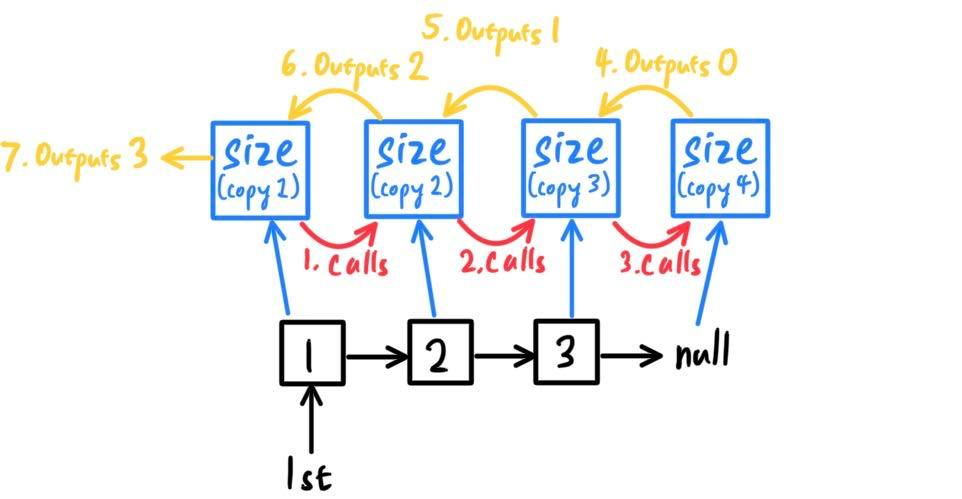
\includegraphics[scale=0.3]{img/size_recursion.jpg}
\end{center}
\end{example}

Note that we must ensure that every recursive call gets closer to the base case, or this may never end. Speaking of runtime, let us state a method to compute the runtime complexity of recursive algorithms. 

\begin{theorem}[Runtime Complexity of Recursive Algorithms]
To compute the runtime complexity, we must consider two things: 
\begin{enumerate}
    \item At what rate are we approaching the base case? 
    \item How long each recursion takes. 
\end{enumerate}
Once we know these two, we can simply multiply them. 
\end{theorem}

\begin{example}[Reverse]
We can reverse a LinkedList with the following recursive algorithm. 
\begin{verbatim}
public static ListNode reverse(ListNode list) {
    if (list == null || list.next == null) {
        return list; 
    }
    ListNode reversedLast = list.next; 
    ListNode reversedFirst = reverse(list.next); 
    reversedLast.next = list; 
    list.next = null; 
    return reversedList; 
}
\end{verbatim}
\end{example}

\begin{example}
The following algorithm 
\begin{verbatim}
public static ListNode rec(ListNode list) {
    if (list == null || list.next == null) {
        return list; 
    }
    ListNode after = rec(list.next); 
    if (list.info <= after.info) {
        list.next = after; 
        return list; 
    }
    return after; 
}
\end{verbatim}
\end{example}

\subsection{Sorting}

As a start, we can sort only ordered things, so we will be talking about arrays and lists (both ArrayLists and LinkedLists). The $\texttt{Java.util}$ implementations sort from least to greatest, sorts in place (i.e. mutates the array rather than creating a new one), and is stable (i.e. does not reorder elements if not needed). 
\begin{enumerate}
    \item $\texttt{Arrays.sort(int[] x)}$ is used to sort arrays and is $O(n \log{n})$ 
    \item $\texttt{Collections.sort(List<> x)}$ is used to sort lists and is $O(n \log{n})$. 
\end{enumerate}

By definition, sorting requires some sort of order $\leq$ defined on a set, and this order can be implemented through a comparable interface, which has a $\texttt{a.compareTo(b)}$ method, which returns a negative integer for $\leq$, $0$ for $=$, and a positive integer for $\geq$. 

\begin{example}
Since strings implement this interface, we can compare them lexicographically, which is the \textbf{natural order} for String objects. 
\begin{enumerate}
    \item $\texttt{"a".compareTo("b")}$ returns $-1$ 
    \item $\texttt{"b".compareTo("b")}$ returns $0$ 
    \item $\texttt{"b".compareTo("a")}$ returns $1$
\end{enumerate}
\end{example}

\begin{example}
We can create a custom class of Blobs and compare them by their names. 
\begin{verbatim}
public class Blob implements Comparable<Blob> {
    String name; 
    String color; 
    int size; 
    
    @Override 
    public int compareTo(Blob other) {
        return this.name.compareTo(other.name); 
    }
}
\end{verbatim}
Therefore, after putting them all into an array, we can call the $\texttt{Arrays.sort}$ method to sort them with our custom $\texttt{compareTo}$ operator. 
\begin{verbatim}
List<Blob> myBlobs = new ArrayList<>(); 
myBlobs.add(new Blob("bo", "blue" 4); 
myBlobs.add(new Blob("al", "red", 2); 
myBlobs.add(new Blob("cj", "green", 1); 
myBlobs.add(new Blob("di", "red", 4); 

System.out.println(myBlobs); 
// [("bo", "blue" 4), ("al", "red", 2), ("cj", "green", 1), ("di", "red", 4)]

Collections.sort(myBlobs); 
System.out.println(myBlobs); 
// [("al", "red", 2), ("bo", "blue" 4), ("cj", "green", 1), ("di", "red", 4)]
\end{verbatim}
\end{example}

If we want to make multiple custom sorting systems that is not the natural order, we have to define a separate helper class implementing a $\texttt{comparator}$ interface. 
\begin{verbatim}
public class Blob implements Comparable<Blob> {
    String name; 
    String color; 
    int size; 
    
    @Override 
    public int compareTo(Blob other) {
        return this.name.compareTo(other.name); 
    }
    
    public class BlobComparator implements Comparator<Blob> {
        @Override 
        public int compare(Blob a, Blob b) {
            int sizeDiff = a.size - b.size; 
            if (sizeDiff != 0) {
                return (-1) * sizeDiff; 
            }
            return a.compareTo(b); 
        }
    }
    
    public static void main(String[] args) {
        \\ assume myBlobs already defined 
        
        System.out.println(myBlobs); 
        // [("bo", "blue" 4), ("al", "red", 2), ("cj", "green", 1), ("di", "red", 4)]
        
        Collections.sort(myBlobs, new BlobComparator()); // custom sorting  
        System.out.println(myBlobs); 
        // [("bo", "blue" 4), ("di", "red", 4), ("al", "red", 2), ("cj", "green", 1)]
    }
}
\end{verbatim}

In summary, comparables allow you to define an natural ordering, while comparators allow you to define other custom orderings. Furthermore, when comparing two $\texttt{a}$ and $\texttt{b}$, comparables are methods on the specific object $\texttt{a.compareTo(b)}$, while comparators are methods on the $\texttt{Comparator}$ object $\texttt{c.compare(a, b)}$. 

\begin{theorem}[Comparator Shorthands]
Here are some comparator shorthands: 
\begin{enumerate}
    \item To create a comparator that compares according to the natural order, we just do 
    \begin{verbatim}
    Comparator<String> c = Comparator.naturalOrder(); 
    c.compare("a", "b") \\ -1 
    c.reversed().compare("a", "b"); \\ 1
    \end{verbatim}
    
    \item To create a comparator that compares according to the length, we just do 
    \begin{verbatim}
    Comparator<String> c = Comparator.comparing(String::length); 
    c.compare("this", "is") \\ 1 
    c.compare("is", "it") \\ 0 
    \end{verbatim}
    
    \item If we want to compare according to the length and then the natural order, then we just do 
    \begin{verbatim}
    Arrays.sort(arr, Comparator.
        comparing(String::length).
            thenComparing(Comparator.naturalOrder())); 
    \end{verbatim}
\end{enumerate}
\end{theorem}

\begin{definition}[Selection Sort]
The \textbf{selection sort} algorithm is an iterative algorithm with the loop invariant that "on iteration $i$, the first $i$ elements are the smallest $i$ elements in sorted order." On iteration $i$, we must find the smallest element from index $i$ onward and swap that with the element at index $i$. 
\begin{verbatim}
public static void selectSort(int[] ar) {
    for (int i = 0; i < ar.length; i++) {
        int minDex = i; 
        for (int j=i+1; j < ar.length; j++) {
            if (ar[j] < ar[minDex]) {
                minDex = j; 
            }
        }
        int temp = ar[i]; 
        ar[i] = ar[minDex]; 
        ar[minDex] = temp; 
    }
}
\end{verbatim}
This is $O(n^2)$. 
\end{definition}

\begin{definition}[MergeSort Algorithm]
An improved version of this algorithm uses a recursive method, which does the steps
\begin{enumerate}
    \item Take an array split it into two halves. 
    \item Sort the first half and then sort the second half. 
    \item Merge the two halves so that the combined total is sorted. 
\end{enumerate}
and has the base case that sorting an array of length 1 is just itself. To do this, we must describe the helper function $\texttt{merge}$, which will merge two sorted arrays into a bigger sorted array. We basically want to loop through each indices of each array and add the smaller element to the new bigger array until we've exhausted all elements in one of the arrays. Then, we just copy the rest of the elements in the other array over. 

Furthermore, we can create a wrapper function $\texttt{mergeSort}$, which helps us initialize the parameters to the recursive call, allowing for more convenience. 
\begin{verbatim}
public static void mergeSort(int[] ar) {
    mergeHelper(ar, 0, ar.length); 
}

public static void merge(int[] ar, int l, int mid, int r) {
    int[] sorted = new int[r - l]; 
    int sDex = 0; int lDex = l; int rDex = mid; 
    while (lDex < mid && rDex < r) {
        if (ar[lDex] <= ar[rDex]) {
            sorted[sDex] = ar[lDex]; 
            lDex++; 
        }
        else {
            sorted[sDex] = ar[rDex]; 
            rDex++; 
        }
        sDex++; 
    }
    if(lDex == mid) {System.arraycopy(ar, rDex, sorted, sDex, r - rDDex); }
    else {System.arraycopy(ar, lDex, sorted, sDex, mid - lDex); }
    System.arraycopy(sorted, 0, ar, l, r - l); 
}

public static void mergeHelper(int[] ar, int l, int r) {
    int diff = r - l; 
    if (diff < 2) {return;}     // base case if 0 or 1 elements 
    int mid = l + diff/2 
    mergeHelper(ar, l, mid);    // recursively sort 1st half 
    mergeHelper(ar, mid, r);    // recursively sort 2nd half 
    merge(ar, l, mid, r);       // merge the 2 sorted parts 
}
\end{verbatim}
There will be $O(\log{n})$ levels of recursion, and for each recursion we will have to run the $\texttt{merge}$ function, which is linear in the number of elements we are sorting ($O(n)$), so the total time complexity of this algorithm is $O(n \log{n})$. We can also determine the \textbf{recurrence relation} of this algorithm as
\[T(N) = T(N/2) + T(N/2) + O(N) = O(N \log{N})\]
\end{definition}

\subsection{Searching}

\begin{definition}[Binary Search]
Given that we have a sorted list (this is important!), we can search for the index of an element in $O(\log{n})$ time. We want the loop invariant "if the target is in the array/list, it is in the range [low, high]." Let us have a list of $N$ elements, and at every step, we either 
\begin{enumerate}
    \item get our desired element and its index, or 
    \item cut down our search space by half
\end{enumerate}
The code can be a bit more general by implementing a generic type $\texttt{T}$. 
\begin{verbatim}
public static <T> int binarySearch(List<T> list, T target, Comparator<T> comp) {
    int low = 0; 
    int high = list.size() - 1; 
    while (low <= high) {
        int mid = (low + high)/2;   // rounds down since integer division
        T midval = list.get(mid); 
        
        int cmp = comp.compare(midval, target); 
        if (cmp < 0) 
            low = mid + 1; 
        else if (cmp > 0) 
            high = mid - 1; 
        else 
            return mid;         // target found 
    }
    return -1;      // target not found 
}
\end{verbatim}
\end{definition}

\section{Trees}

\subsection{Stacks, Queues, and Priority Queues}

\begin{definition}[Stacks]
A \textbf{stack} is an abstract data structure represented as a \textbf{Last-In-First-Out (LIFO) list}, which implements the following methods given stack $\texttt{st}$, which we can initialize with 
\begin{verbatim}
    Stack<String> st = new Stack<>(); 
    for (String s : strs) { st.push(s); }
    while (! st.isEmpty()){ System.out.println(st.pop()); }
\end{verbatim}
\begin{enumerate}
    \item $\texttt{st.add(Object element)}$ adds to the top of the stack, which is $O(1)$ 
    \item $\texttt{st.pop()}$ removes the element that is at the top of the stack, which is $O(1)$, and returns whatever is popped out. 
\end{enumerate}
Remember that this is just a list and so anything we can do with a stack we can do with a list. What makes the stack so useful is the way the list is implemented. We can literally imagine the elements of this list as "stack." If you want to remove something from the stack, of course you have to remove the top element. 
\end{definition}

\begin{definition}[Queue]
A \textbf{queue} is an abstract data structure represented as a \textbf{First-In-First-Out (FIFO) list}, which implements the following methods given queue $\texttt{q}$, which we can initialize with 
\begin{verbatim}
    Queue<String> q = new LinkedList<>(); 
    for (String s : strs) { q.add(s); }
    while (! q.isEmpty()) { System.out.println(q.remove()); }
\end{verbatim}
Note that LinkedList implements the Queue interface. 
\begin{enumerate}
    \item $\texttt{q.add(Object element)}$ adds to the top of the queue, referred to as \textbf{enqueue}. 
    \item $\texttt{q.remove()}$ removes the first element in the queue, referred to as \textbf{dequeue}. 
\end{enumerate}
This is just like how a queue works. Whatever has been waiting in the queue the longest is the one that is removed first. 
\end{definition}

For now, we will abstractly think that a priority queue acts as a sorted list (though it is actually implemented as a binary heap). 

\begin{definition}[Priority Queues]
A priority queue simply adds things according to their priority. Every time we add an element, it looks at where the element should go to keep the list sorted. If we want to dequeue, then we just remove the first element of the list. 
\begin{verbatim}
    PriorityQueue<String> pq = new PriorityQueue<>();
    pq.add("ac"); 
    pq.add("c"); 
    pq.add("bdf"); 
    while(! pq.isEmpty()) { System.out.println(pq.remove()); }
    // ac   bdf  c
\end{verbatim}
But depending on the comparator what we use, the priority queue sorts it in a different manner. 
\begin{verbatim}
    PriorityQueue<String> pq = new PriorityQueue<>(Comparator.comparing(String::length)); 
    pq.add("ac"); 
    pq.add("c"); 
    pq.add("bdf"); 
    while(! pq.isEmpty()) { System.out.println(pq.remove()); }
    // c   ac   bdf
\end{verbatim}
\begin{enumerate}
    \item $\texttt{pq.add(Object element)}$ is $O(\log(N))$
    \item $\texttt{pq.remove()}$ is $O(\log(N))$ 
    \item $\texttt{pq.peek()}$ returns the minimal element and is $O(1)$
    \item $\texttt{pq.size()}$ returns number of elements and is $O(1)$
\end{enumerate}
\end{definition}

\subsection{Binary Trees}

Let us compare the HashSet/Map and the TreeSet/Map. The purpose of Hashing is to "find" and add elements quickly. 
\begin{enumerate}
    \item This means that add, contains, put, and get are all amortized $O(1)$ (under Simple Uniform Hashing Assumption). The TreeSet/Map have all operations add, contains, put, get are $O(\log(N))$, which is slower, but is not amortized. 
    \item Trees are sorted, while Hashes are not, and so we can get a range of Tree values in sorted order efficiently, but not for Hashes. 
\end{enumerate}

A Node for trees is represented with the following class. 
\begin{verbatim}
public class TreeNode {
    TreeNode left; 
    TreeNode right; 
    String info; 
    
    TreeNode (String s) {
        info = s; 
    }
    
    TreeNode(String s, TreeNode llink, TreeNode rlink) {
        info = s; 
        left = llink; 
        right = rlink; 
    }
}
\end{verbatim}

A tree looks pictorially like this: 
\begin{center}
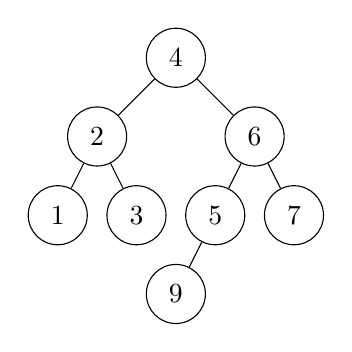
\begin{tikzpicture}[  every node/.style={    circle,    minimum size=0.75cm,    draw,    text centered,    anchor=center  }]
  \node (4) at (0,0) {4};
  \node (2) at (-1,-1) {2};
  \node (6) at (1,-1) {6};
  \node (1) at (-1.5,-2) {1};
  \node (3) at (-0.5,-2) {3};
  \node (5) at (0.5,-2) {5};
  \node (7) at (1.5,-2) {7};
  \node (9) at (0, -3) {9}; 
  \draw (4) -- (2);
  \draw (4) -- (6);
  \draw (2) -- (1);
  \draw (2) -- (3);
  \draw (6) -- (5);
  \draw (6) -- (7); 
  \draw (5) -- (9); 
\end{tikzpicture}
\end{center}
Some terms: 
\begin{enumerate}
    \item The root of the tree is the top node, which is $4$
    \item The leaf of the tree are nodes that do not have a left nor right subchild. 
    \item A path is any path from one node to another node. A simple path is a path that doesn't cross the same edge twice 
    \item The height of a node is the length of the longest downward path to a leaf from that node. 
    \item The depth of a node is the number of edges from the root to the node. 
\end{enumerate}

\subsubsection{Algorithms for Binary Tree}

\begin{theorem}[Print All Nodes in A Binary Tree]
Here are three ways to recursively traverse a tree. The difference is in where the nonrecursive part is. Let us have a binary tree from above. 
\begin{enumerate}
    \item This tells us to print everything on the left of the node, then print the node, and then print everything on the right. 
    \begin{verbatim}
    void inOrder(TreeNode t) {
        if (t != null) {
            inOrder(t.left);
            System.out.println(t.info); 
            inOrder(t.right); 
        }
    }
    // 1, 2, 3, 4, 9, 5, 6, 7
    \end{verbatim}
    
    \item This tells us to print the node itself first, then print all the ones on the left, and then print all the ones on the right. 
    \begin{verbatim}
    void preOrder(TreeNode t) {
        if (t != null) {
            System.out.println(t.info); 
            preOrder(t.left); 
            preOrder(t.right); 
        }
    }
    // 4, 2, 1, 3, 6, 5, 9, 7
    \end{verbatim}
    
    \item This tells us to print all the nodes on the left, then all ones on the right, and then the node itself. 
    \begin{verbatim}
    void postOrder(TreeNode t) {
        if (t != null) {
            postOrder(t.left); 
            postOrder(t.right); 
            System.out.println(t.info); 
        }
    }
    // 1, 3, 2, 9, 5, 7, 6
    \end{verbatim}
\end{enumerate}
\end{theorem}

\begin{theorem}[Storing All Nodes in a List]
Now if we want to store them all in a list, then this recursive strategy will not work, since if we create a list inside the function body, then we will have a bunch of lists floating around in memory. Therefore, we want to initialize a list outside of the entire function, and store that entire thing within a wrapper function. The $\texttt{inOrder}$ takes in also a reference to a list that it will be adding to. 
\begin{verbatim}
public ArrayList<String> visit(TreeNode root) {
    ArrayList<String> list = new ArrayList<>(); 
    inOrder(root, list); 
    return list; 
}

private void inOrder(TreeNode root, ArrayList<String> list) {
    if (root != null) {
        inOrder(root.left, list); 
        list.add(root.info); 
        inOrder(root.right, list); 
    }
}
\end{verbatim}
\end{theorem}

\begin{definition}[Finding Height of Node]
The height of a node is the longest downward path to a leaf from that node, so its height would be the maximum of the two heights of its children. A null node would have height $-1$, which is our base case. 
\begin{verbatim}
public int getHeight(TreeNode root) {
    if (root == null) { return -1; }
    return 1 + Math.max(getHeight(root.left), getHeight(root.right)); 
}
\end{verbatim}
\end{definition}

\begin{definition}[Finding Depth of Node]
The depth is quite hard to find recursively, but if we have a reference to the parent, then we can write 
\begin{verbatim}
int depth(TreeNode node) {
    if (node == null) {
        return -1;
    } else {
        return 1 + depth(node.parent);
    }
}
\end{verbatim}
\end{definition}



\subsubsection{Binary Search Tree}

\begin{definition}[Binary Search Tree]
A binary tree is a \textbf{binary search tree} if for every node, the left subtree values are all less than the node's value, and the right subtree values are all greater than the node's value. That is, the nodes are in order, and if we called $\texttt{inOrder(root)}$ on the tree, then we would get a sorted list, which allows for efficient search. 
\end{definition}

We could then search recursively with the following: 
\begin{verbatim}
public boolean contains(TreeNode tree, String target) {
    if (tree == null) return false; 
    int result = target.compareTo(tree.info); 
    if (result == 0) return true; 
    if (result < 0) return contains(tree.left, target); 
    return contains(tree.right, target); 
}
\end{verbatim}

or iteratively with
\begin{verbatim}
public static boolean contains(TreeNode node, String target) {
    while (node != null) {
        int comp = node.info.compareTo(target); 
        if(comp == 0) return true; 
        else if (comp > 0) node = node.left; 
        else node = node.right; 
    }
    return false; 
}
\end{verbatim}

Adding elements to a binary search tree is also very similar. But note that the order in which we add elements to the binary search tree will matter, since it can either make the tree \textbf{balanced} or \textbf{unbalanced}. 
\begin{figure}[h]
\centering
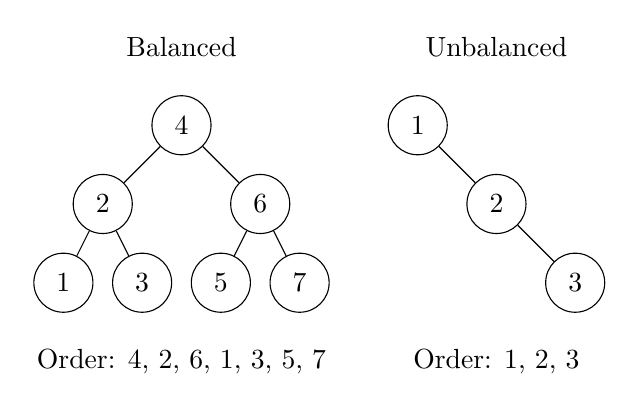
\begin{tikzpicture}[ integer/.style={    draw,    circle,    minimum size=0.75cm,    inner sep=0pt,    text centered,    anchor=center  }]
  % Balanced tree
  \node[integer] (4) at (0,0) {4};
  \node[integer] (2) at (-1,-1) {2};
  \node[integer] (6) at (1,-1) {6};
  \node[integer] (1) at (-1.5,-2) {1};
  \node[integer] (3) at (-0.5,-2) {3};
  \node[integer] (5) at (0.5,-2) {5};
  \node[integer] (7) at (1.5,-2) {7};
  \draw (4) -- (2);
  \draw (4) -- (6);
  \draw (2) -- (1);
  \draw (2) -- (3);
  \draw (6) -- (5);
  \draw (6) -- (7);

  % Caption for balanced tree
  \node at (0,1) {Balanced};
  \node at (0,-3) {Order: 4, 2, 6, 1, 3, 5, 7};

  % Unbalanced tree
  \node[integer] (1') at (3,0) {1};
  \node[integer] (2') at (4,-1) {2};
  \node[integer] (3') at (5,-2) {3};
  \draw (1') -- (2');
  \draw (2') -- (3');

  % Caption for unbalanced tree
  \node at (4,1) {Unbalanced};
  \node at (4,-3) {Order: 1, 2, 3};
\end{tikzpicture}
\caption{Comparison of balanced and unbalanced binary trees}
\label{fig:trees}
\end{figure}
In a balanced case, contains/add will be $O(\log(N))$, while in an unbalanced case, we will have $O(N)$. 


\subsection{Greedy Algorithms, Huffman}

A \textbf{greedy algorithm} is an approach for solving a problem by selecting the best option available at the moment. They are useful because they may be optimal, they may not be optimal but work very well in practice, and they are easier to implement for starting out. It turns out that many large-scale machine learning models, like neural nets, are optimized using greedy algorithms (e.g. gradient descent). 

\begin{example}
In the Knapsack problem, we have \$10 and want to buy things at a market that maximizes our value. Say that we have an \$1 apple with value 2, a \$1 banana with value 1, and a \$10 pizza with value 10. Then, a greedy algorithm will make sure to first buy all things with the highest value-to-cost ratio. 
\end{example}

Now, let's talk about \textbf{Huffman encoding}. We already know about the ASCII encoding that encodes characters in $7$ bits, for a total of $2^7$ possibilities. The extended ASCII uses $8$ bits, but all of these things use something called \textbf{fixed-length encoding} which uses a constant number of bits to encode any character. To compress something, we want to use \textbf{variable-length encoding}. 

To decode something, the mapping from the characters to the bits must be injective, so we can define an inverse over its image. It turns out that if we an encoding for 3 characters, say 
\[a \mapsto 1, b \mapsto 10, c \mapsto 11\]
then decoding $1011$ is ambiguous since $1$ is a prefix of the encoding for $c$. Therefore, we do not want one encoding to be the prefix of another. It turns out that we can avoid this conflict by encoding everything as a binary tree and setting all encodings as leaf nodes. 
\begin{center}
    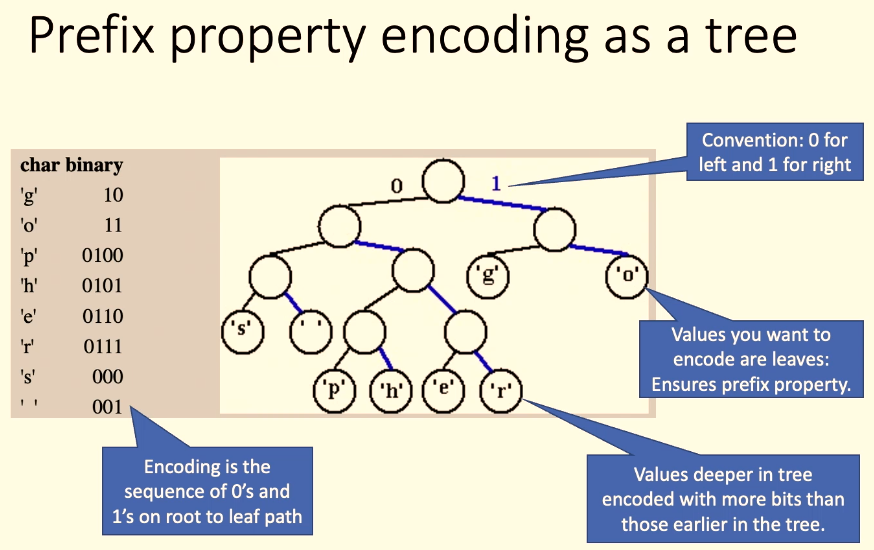
\includegraphics[scale=0.5]{img/Tree_Encoding.png}
\end{center}
This makes sense since an encoding will be a prefix of another if and only if it is a parent of another. Furthermore, a greater depth of a character in the tree corresponds to a longer encoding. So, Huffman encoding tries to convert shorter characters to longer leaves and less recurrent characters into longer encodings. To decode a string of bits using a tree, we read the bit at a time to traverse left or right edge. When we reach a leaf, we decode the character and restart at root. 

Now, we describe the greedy algorithm for building an optimal variable length encoding tree. 
\begin{enumerate}
    \item We take the document and compute the frequencies of all characters that we want to encode. We want to less frequent characters to be lower on the tree, and so we will build the tree up from the leaves. 
    \item We iteratively choose the lowest weight nodes to connect up to a new node with weight = sum of children. 
\end{enumerate}
We implement this using a priority queue. 

\begin{example}
Let us go do an example of where we have the characters and frequencies 
\[a \mapsto 30, \; b \mapsto 20, \; c \mapsto 10, \; d \mapsto 15, \; e \mapsto 40\]
Then, we have the following steps: 
\begin{enumerate}
    \item We write out them as leaf nodes with the values $30, 20, 10, 15, 40$. We take the smallest of the frequencies and sum them up: $10 + 15 = 25$. 
    \begin{center}
        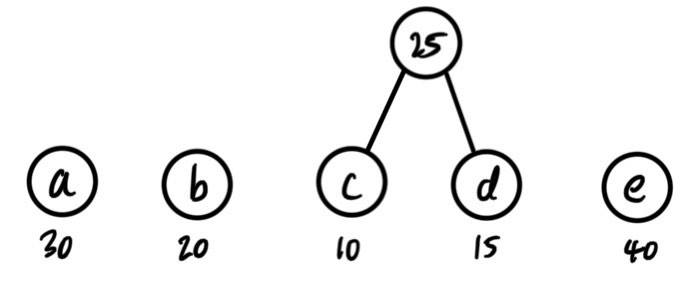
\includegraphics[scale=0.3]{img/step_1.jpg}
    \end{center}
    \item We have the values $30, 20, 25, 40$. We sum the smallest two frequencies: $20 + 25 = 45$. 
    \begin{center}
        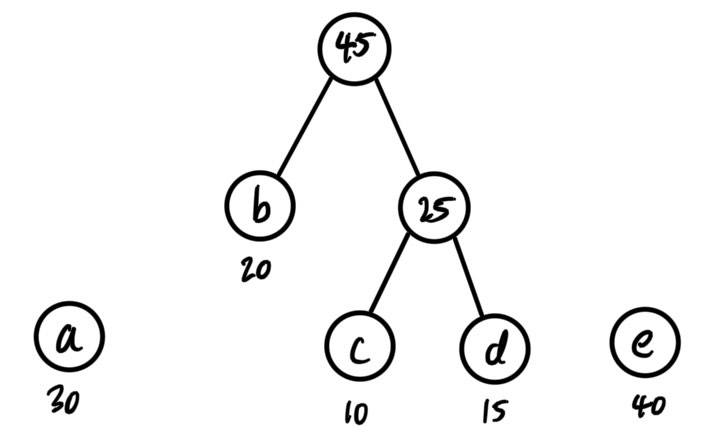
\includegraphics[scale=0.3]{img/step_2.jpg}
    \end{center}
    \item We have the values $30, 45, 40$. We sum the smallest two frequencies: $30 + 40 = 70$. 
    \begin{center}
        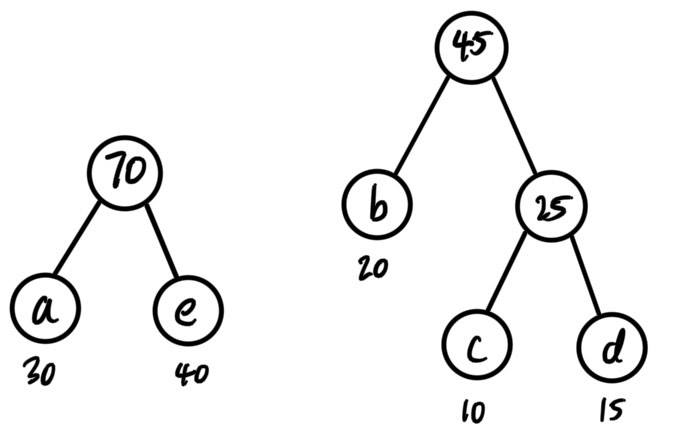
\includegraphics[scale=0.3]{img/step_3.jpg}
    \end{center}
    \item We have the values $70, 45$. We sum them up to get the complete tree. 
    \begin{center}
        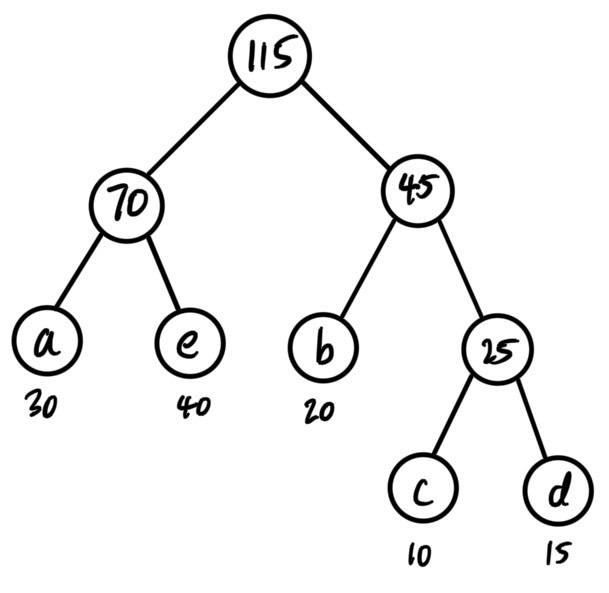
\includegraphics[scale=0.3]{img/step_4.jpg}
    \end{center}
\end{enumerate}
\end{example}

\begin{theorem}
If we have a document of $N$ total characters and $M$ unique characters, the number of nodes in the Huffman tree, in complexity notation, is 
\[O(M)\]
Clearly, this has nothing to do with $N$. Note that we have $M$ leaf nodes, and in each iteration, we connect 2 nodes up to a parent. Therefore, the number of nodes to connect up decreases by 1 per iteration, and we create a new node per iteration. Since there are $M - 1$ iterations, we add one node, so there will be $M + M - 1 = O(n)$ nodes in the binary tree. 
\end{theorem}

\subsection{Binary Heaps}

\begin{definition}[Binary Heap]
A \textbf{binary heap} is a binary tree satisfying the following structural invariants: 
\begin{enumerate}
    \item Maintain the \textbf{heap property} that every node is less than or equal to its successors, and 
    \item The \textbf{shape property} that the tree is complete (full except perhaps last level, in which case it should be filled from left to right. 
\end{enumerate}
We should conceptually think of a binary heap as an underlying binary heap, but it is actually usually implemented with an array, and we can create a map from the heap to the array with the following indices. 
\begin{center}
    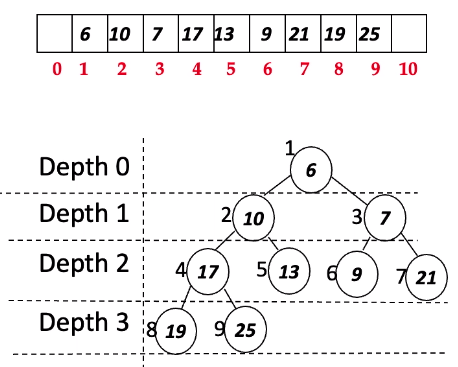
\includegraphics[scale=0.5]{img/binary_heap.png}
\end{center}
When 1-indexing, for node with index $k$, the left child is index $2k$, the right child is index $2k + 1$, and the parent is index $k/2$ (where this is integer division). 
\end{definition}

Implementing peek is easy, since we just return the first index, but it can be quite tricky to maintain this invariant after an arbitrary sequence of add/remove operations. 
\begin{enumerate}
    \item To add values to a heap, we add to the first open position in the last level of the tree (to maintain the shape property), and then swap with the parent is the heap property is violated. If we are swapping with the parent at most $\log(N)$ times, then the add property has $O(\log(N))$ complexity. 
    \begin{center}
        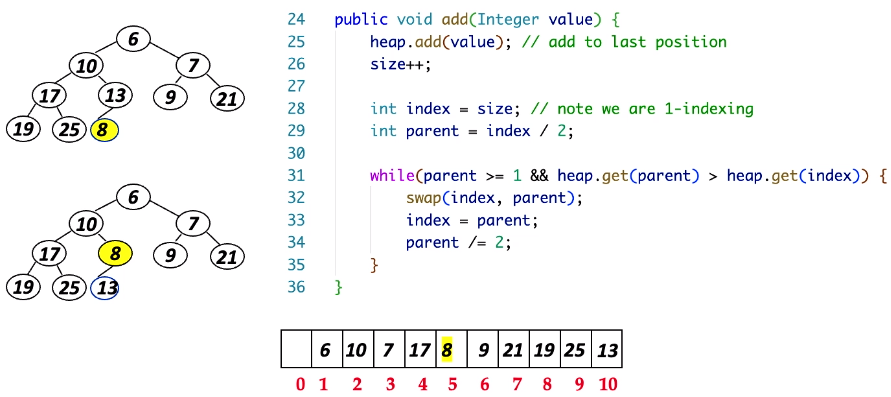
\includegraphics[scale=0.5]{img/heap_add_implementation.png}
    \end{center}
    
    \item We remove the first (minimal) value, we first replace the root with the last node in the heap, and while the heap property is violated, we swap with the smaller child. There are two choices, the left or right child, in which we can swap. But we must always swap with the \textbf{smaller child}, since we swapped with the bigger child, then this bigger child would be larger than the smaller one, violating the heap property. Since a complete binary tree always has height $O(\log(N))$, remove also "traverses" one root-leaf path, and so its runtime complexity is $O(\log(N))$, too. 
    \begin{center}
        % \includegraphics[scale=0.5]{}
    \end{center}
    
    \item The decreaseKey operation just takes an arbitrary node and decreases its value to some other integer. In this case, it wouldn't violate the shape property, and to restore the heap property, we just put swap it with its parent if the new value is smaller than its parent, making this operation $O(\log(N))$. 
\end{enumerate}

\subsection{Red-Black Trees}

Now, we have learned how we can implement a priority queue using a binary heap. This is also possible to use a binary search tree, since it's easy to get the minimal element for adding and removing, but there are three things that make it difficult: 
\begin{enumerate}
    \item all elements must be unique 
    \item it is not array-based, and so uses more memory and higher constant factors on runtime 
    \item it is much harder to implement with guarantees that the tree will be balanced. This makes it difficult since if we want to search through a balanced BST, it is $O(\log(N))$, but if it turns out to be unbalanced, then it is $O(N)$. 
\end{enumerate}
Therefore, while a balanced tree may be efficient on average, in the worst case the linear complexity is not tolerable. Therefore, we must implement a binary search tree that will do extra work to ensure that they are approximately balanced. 

\begin{definition}[Red-Black Tree]
\textbf{Red-Black Trees} are binary search trees that satisfy the following properties: 
\begin{enumerate}
    \item Every node is red or black 
    \item The root is black 
    \item A red node cannot have red children 
    \item From a given node, all paths to null descendants must have the same number of black nodes. (Null is considered to be a black node)
    \item remember that it must be a binary search tree! 
\end{enumerate}
\begin{center}
    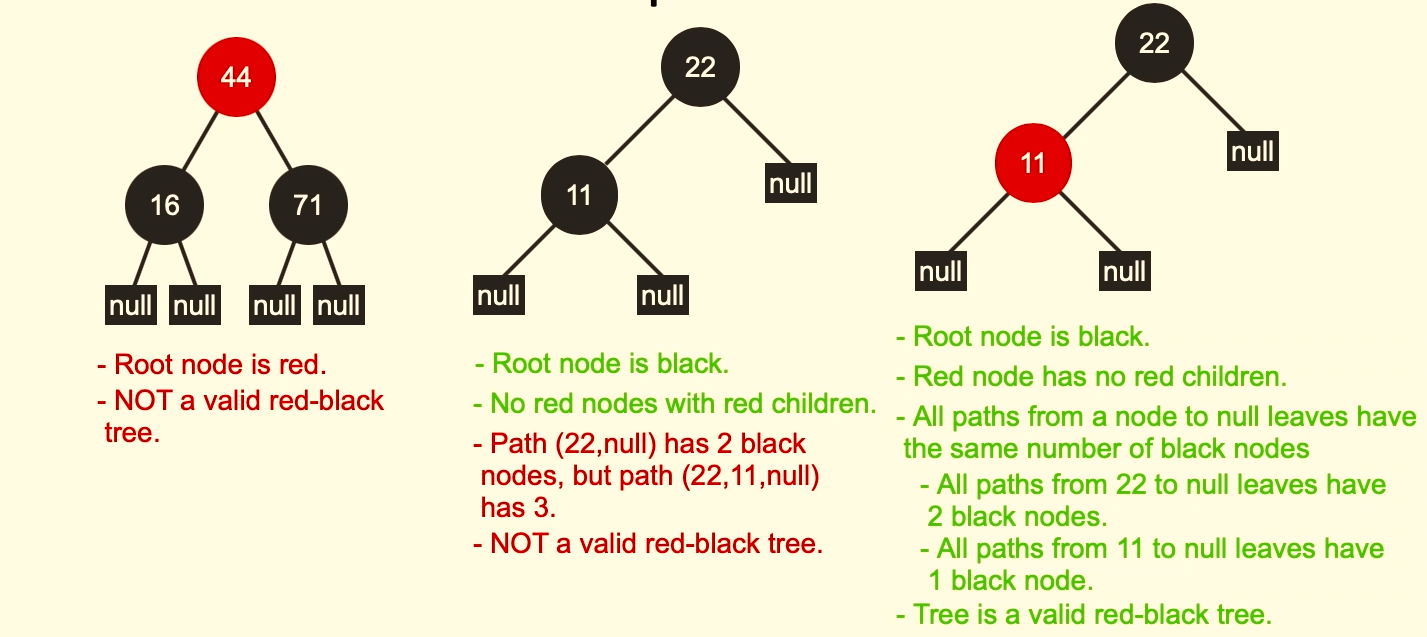
\includegraphics[scale=0.4]{img/red_black_trees.png}
\end{center}
\end{definition}

Note that there are binary search trees that cannot be turned into a red-black tree. 
\begin{center}
    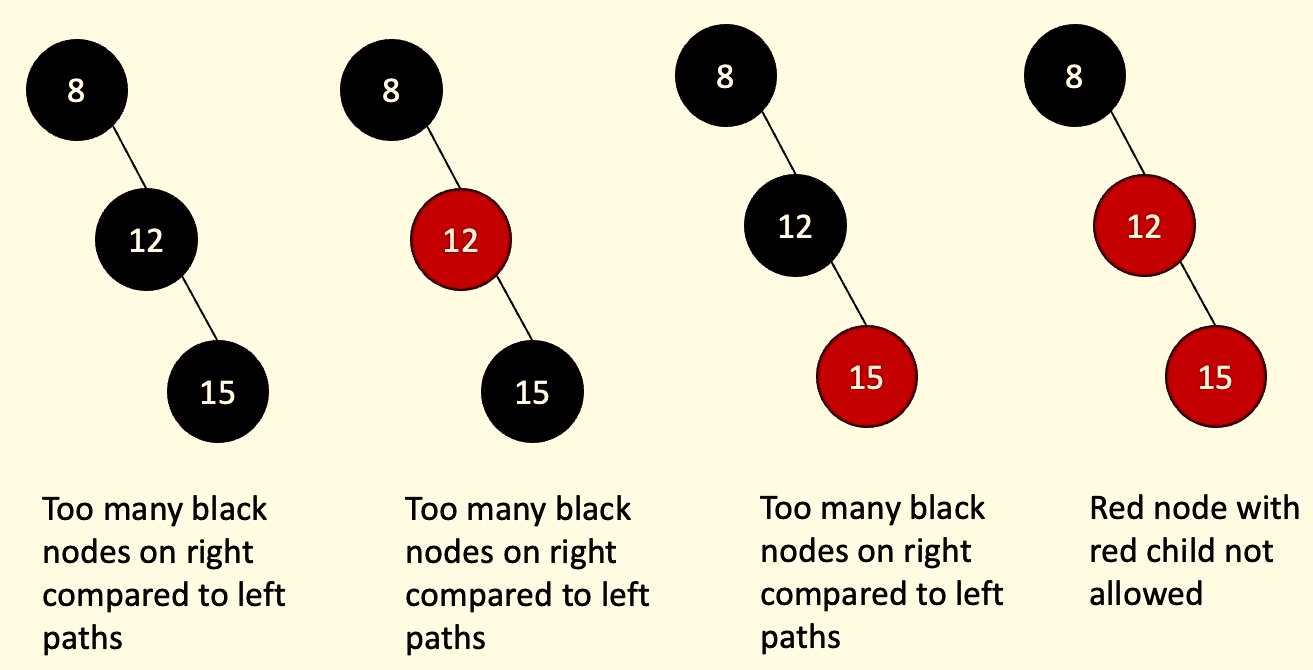
\includegraphics[scale=0.3]{img/impossible_red_black.png}
\end{center}
This is intentional because red-black tree properties guarantee approximate balance. If we can turn a binary search tree into a red-black tree, then it logically follows that the original BST was approximately balanced. Note that a red black tree does not make searching asymptotically faster in any way; it just takes care of the worst-case. 

Remember that red black trees are also just binary search trees: 
\begin{enumerate}
    \item contains (search) method is the exact same thing as BST 
    \item The add method needs to be slightly modified, since after we add, we need to make sure that the resulting tree is a red-black tree. This is done in three steps: 
    \begin{enumerate}
        \item Run the regular BST add 
        \item Color the new node red 
        \item Fix the tree to reestablish red-black tree properties. This is extremely complicated with different cases, but it all essentially uses some sort of recoloring and a (right or left) rotation of the tree. 
    \end{enumerate}
\end{enumerate}


\section{Graphs}

\begin{definition}[Graph]
A \textbf{graph} is a data structure for representing connections among items an dconsists of vertices connected by edges. It consists of a \textbf{vertex} (or node) and an \textbf{edge}. It can be directed or undirected. A \textbf{simple graph} there is at most one undirected edge between nodes (or 2 directed). Therefore, given that $N$ is the number of vertices and $M$ the number of edges, we have 
\[M \leq N^2\]
for a simple graph. A \textbf{simple path} is a sequence of unique vertices where subsequent nodes are connected by edges, and the path doesn't repeat itself. 
\end{definition}

\begin{definition}[Adjacency List/Matrix]
Given a graph, we can completely represent it with a list of adjacent vertices for each vertex or an adjacency matrix. 
\begin{center}
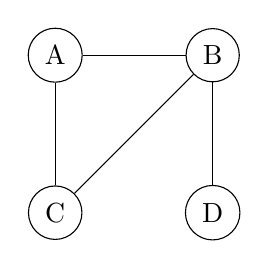
\begin{tikzpicture}
  \node[circle, draw] (C) at (0,0) {C};
  \node[circle, draw] (D) at (2,0) {D};
  \node[circle, draw] (B) at (2,2) {B};
  \node[circle, draw] (A) at (0,2) {A};

  \draw (A) -- (B);
  \draw (B) -- (C);
  \draw (A) -- (C);
  \draw (B) -- (D);
\end{tikzpicture}
\end{center}
An adjacency list would look something like this 
\[
\begin{aligned}
A &: B, C \\
B &: A, C, D \\
C &: A, B \\
D &: B
\end{aligned}
\]
and the adjacency matrix looks like this: 
\begin{center}
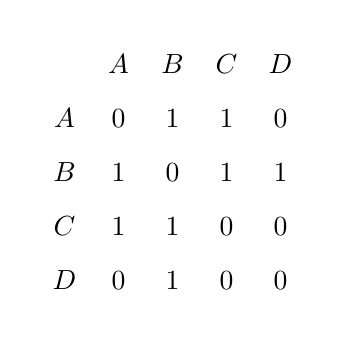
\begin{tikzpicture}
  \matrix[matrix of math nodes, nodes in empty cells,          column sep=-\pgflinewidth, row sep=-\pgflinewidth,          nodes={minimum size=7mm, anchor=center, outer sep=0pt}] (adjacency) {
    & |(a)| A & |(b)| B & |(c)| C & |(d)| D \\
    |(A)| A & 0 & 1 & 1 & 0 \\
    |(B)| B & 1 & 0 & 1 & 1 \\
    |(C)| C & 1 & 1 & 0 & 0 \\
    |(D)| D & 0 & 1 & 0 & 0 \\
  };
\end{tikzpicture}
\end{center}
Adjacency matrices can be memory wasteful if the graph is sparse, and for fast lookup of information in adjacency lists, we can implement a double hashing mechanism ($\texttt{hashMap<Vertex, HashSet<Vertex>>}$). 
\end{definition}

\subsection{Depth First Search (DFS)}

DFS basically traverses 


\begin{theorem}[Recursive DFS]
Now, in order to traverse this graph, we basically want to make an algorithm that starts at a node, prints it value, and then goes to all of its neighbors (which we can access through the adjacency list) to print them out. Thus, this is by nature recursive. We don't want the algorithm to loop around printing nodes infinitely often, so we must create a base case that tells the algorithm to not print out a node. It makes sense to create a set of visited nodes, which we can add to whenever we reach a new node. So, if we ever come onto a node that we have visited, we can just tell the function to do nothing. 

Now if we want to print out all the nodes of a general graph, we can do the following:
\begin{verbatim}
    public static void dfs(char start) {
        if (!visited.contains(start)) {                // if already visited, backtrack
            visited.add(start);                         // else, visit this node 
            System.out.println(start);                  // print it out
            for (char neighbor : aList.get(start)) {
                dfs(neighbor);                          // and explore its neighbors 
            }
        }
    }   
\end{verbatim}
\end{theorem}

\begin{theorem}[Iterative DFS]
Though recursion really makes this simple, we can construct an iterative approach that uses stacks. Note that in recursion, we are really making a call stack of different functions. We can be explicit about this by actually implementing a stack, which would store all the nodes that we have discovered, but not yet explored from )i.e. all the current nodes). At each iteration, we would pick a node to continue exploring, and since this is a DFS, we would want to implement a LIFO stack so that the last element we input in is the first thing that we should explore from, i.e. we always explore from the last node discovered. 
\begin{verbatim}
    public static void dfs(char start) {
        Stack<Character> toExplore = new Stack<>(); 
        char current = start; 
        toExplore.add(current); 
        visited.add(current); 
        
        while (!toExplore.isEmpty()) {
            current = toExplore.pop();                  // explore from most recently discovered node
            for (char neighbor : aList.get(current)) {  // look at all neighbors of current node 
                if (!visited.contains(neighbor)) {      // if we haven't seen them before...
                    previous.put(neighbor, current);    // note how we got here 
                    visited.add(neighbor);              // note that we have seen
                    toExplore.push(neighbor);           // mark to explore later
                }
            }
        }
    }
\end{verbatim}
The runtime complexity of this search is $O(N + M)$ because first, the while loop loops at most over the $N$ nodes. The for loop may loop over $M$ edges, but this is a bit pessemistic in bound. Rather, we can view it as looping over neighbors of each node at most exactly once, and so it considers every edge twice, meaning that the for loop will get called $2M$ times in the entire algorithm. So $N + 2M = O(N + M)$. 
\end{theorem}


\begin{example}[DFS in a Maze]
We can represent a grid graph, like a maze, with a two dimensional array that stores whether it is connected north, east, south, and west, where boolean of true represents that there is a wall, and false means there isn't a wall (so connected). 
\begin{center}
    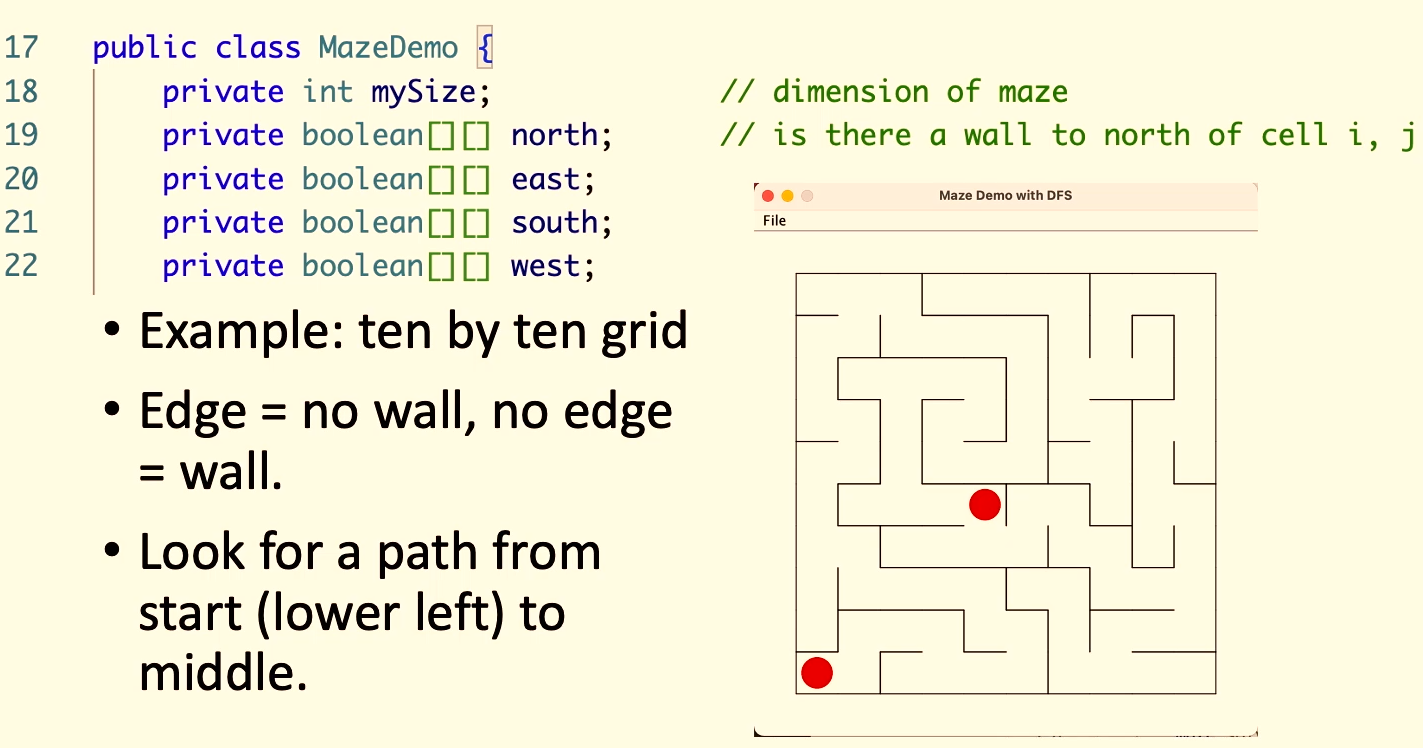
\includegraphics[scale=0.4]{img/grid_graph.png}
\end{center}
But remember that in a tree traversal, we recursively searched down and down until we hit a null node, in which case we backtrack up to look in another branch. For graphs, this is a bit more complicated, since we could go in loops. Therefore, we want to keep track of all the visited nodes to avoid infinite recursion. We have three base cases: 
\begin{enumerate}
    \item If we search off the grid, then this is not a valid path 
    \item If we already explored here, then we don't want to repeat it 
    \item If we reached the goal of the maze, then we output the length of the path. 
\end{enumerate}
The recursive case would take each node and recurse on its 4 adjacent neighbors, if they are connected. So, the entire function, which takes in a location $(x, y)$ in the grid and the depth that it took to traverse to this point, would look like this: 
\begin{verbatim}

private boolean[][] visited; 

private int solveDFS(int x, int y, int depth) {
    if (x == 0 || y == 0 || x == mySize + 1 || y == mySize + 1) {
        return 0; 
    }
    if (visited[x][y]) return 0; 
    
    visited[x][y] = true; 
    
    if (x == mySize/2 && y == mySize/2) {
        return depth; 
    }
    
    if (!north[x][y]) { // if there is no wall above
        int d = solveDFS(x, y + 1, depth + 1); 
        if (d > 0) return d; 
    }
    if (!east[x][y]) {
        int d = solveDFS(x + 1, y, depth + 1); 
        if (d > 0) return d; 
    }
    if (!south[x][y]) {
        int d = solveDFS(x, y - 1, depth + 1); 
        if (d > 0) return d; 
    }
    if (!west[x][y]) {
        int d = solveDFS(x - 1, y, depth + 1); 
        if (d > 0) return d; 
    }
}
\end{verbatim}
Note that this algorithm recurses on each of the $N$ nodes $4$ times (for each direction, and each recursive call is $O(1)$), so the complexity is $O(N)$. 
\end{example}


\subsection{Breadth First Search (BFS)}

Note that the main idea of DFS is to always explore a new adjacent vertex if possible, and if not, then backtrack to the most recent vertex adjacent to an unvisited vertex and continue. On the contrary, the main idea of BFS is to explore \textit{all} your neighbors before you visit any of your neighbors' neighbors. It exhaustively searches for the closest regions of your search space before you look any further. Unlike DFS, which finds the some arbitrary path to a node, BFS finds the shortest (perhaps nonunique) path to a node. 

\begin{definition}[Iterative BFS]
This can be done simply by using a queue. Note that a queue is an interface, so we must use the Linked List implementation. 
\begin{verbatim}
    public static void dfs(char start) {
        Queue<Character> toExplore = new LinkedList<>(); 
        char current = start; 
        toExplore.add(current); 
        visited.add(current); 
        
        while (!toExplore.isEmpty()) {
            current = toExplore.pop();                  // explore from most recently discovered node
            for (char neighbor : aList.get(current)) {  // look at all neighbors of current node 
                if (!visited.contains(neighbor)) {      // if we haven't seen them before...
                    previous.put(neighbor, current);    // note how we got here 
                    visited.add(neighbor);              // note that we have seen
                    toExplore.push(neighbor);           // mark to explore later
                }
            }
        }
    }
\end{verbatim}
\end{definition}

\begin{definition}[Search Trees]
Once we have traversed a graph using BFS or DFS, we can label the directed path that this traversal algorithm takes into a \textbf{search tree}. If we look at the search trees generated by DFS and BFS, we can see that the path from A to C is always shorter for BFS than for DFS. 
\begin{center}
    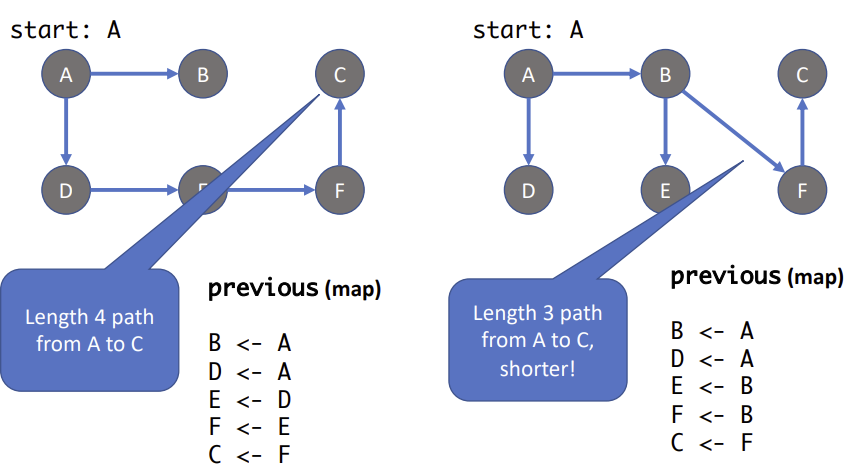
\includegraphics[scale=0.4]{img/search_trees.png}
\end{center}
\end{definition}



\subsection{Shortest Paths and Dijkstra's Algorithm}

\begin{definition}[Weighted Graph]
A \textbf{weighted graph} just has some weights to each of the edges, which can represent multiple things, like distance, cost, or probabilities. 
\begin{center}
    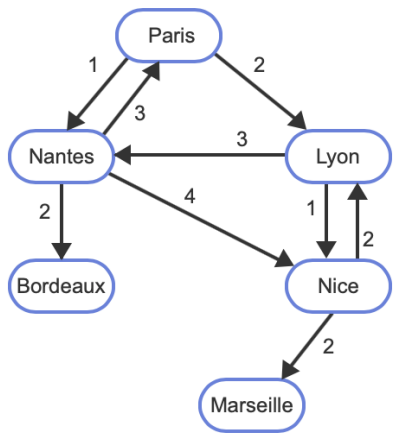
\includegraphics[scale=0.5]{img/weighted_graph.png}
\end{center}
\end{definition}

Remember that BFS gives the shortest paths in \textit{unweighted graphs}. We can generalize BFS to account for weighted graphs, called Dijkstra's algorithm, which doesn't implement queues, but \textit{priority queues}. 

\begin{theorem}[Dijkstra's Algorithm]
The algorithm basically starts at a node, and explores \textit{first} the closest nodes to the start node, called $\texttt{start}$. It does this by recording the shortest distance that it took to travel to this node from the start node. This is implemented in a $\texttt{Map}<Character, Integer>$, which we will call $\texttt{dist}$ for example. Furthermore, we want a $\texttt{PriorityQueue}$ called $\texttt{exp}$ that tells us which nodes that we need to explore next. Let us have a minimal example: 
\begin{center}
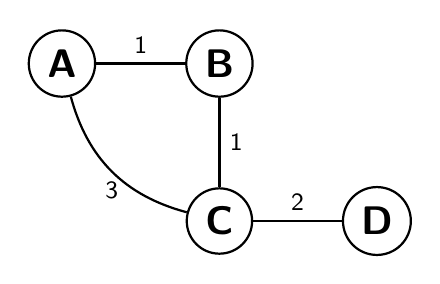
\begin{tikzpicture}[auto,node distance=2cm, thick,main node/.style={circle,draw,font=\sffamily\Large\bfseries}]

  \node[main node] (A) {A};
  \node[main node] (B) [right of=A] {B};
  \node[main node] (C) [below of=B] {C};
  \node[main node] (D) [right of=C] {D};

  \path[every node/.style={font=\sffamily\small}]
    (A) edge node [above] {1} (B)
    (B) edge node [right] {1} (C)
    (A) edge [bend right] node [below] {3} (C)
    (C) edge node [above] {2} (D);
\end{tikzpicture}
\end{center}
\begin{enumerate}
    \item We start at a node $A$, which has distance $0$ (since the distance from $A$ to $A$ is $0$). So, $A$ is $\texttt{current}$, and we have 
    \begin{verbatim}
        dist        exp 
        A -> 0      A 
    \end{verbatim}
    \item We explore from $A$ since that is the first in our Priority Queue. We want to look at all neighbors of the node ($B, C$) and compute their distances from $\texttt{start}$ by adding the distances from $\texttt{start}$ to $\texttt{current}$ and $\texttt{current}$ to the neighbor. So, we have 
    \begin{verbatim}
        dist        exp 
        A -> 0      B
        B -> 1      C 
        C -> 3      
    \end{verbatim}
    
    \item We explore from $B$, since that is first in our Priority Queue. We look at all neighbors of the node ($A, C$). The new distance to $A$ is $d(A, B) + d(B, A) = 2$, so we do not update it. The new distance to $C$ is $d(A, B) + d(B, C) = 2$ and is shorter than the current distance of $3$, so we update it. 
    \begin{verbatim}
        dist        exp 
        A -> 0      C
        B -> 1      
        C -> 2      
    \end{verbatim}
    
    \item We explore from $C$, since that is first in our priority queue. We look at all neighbors of the node ($A, B, D$). The new distance to $A$ is $d(A, C) + d(C, A) = 2 + 3 = 5$, so no update. The new distance to $B$ is $d(A, C) + d(C, B) = 2 + 1 = 3$, so no update. $D$ has not been explored before, so we we add its distance of $d(A, C) + d(C, D) = 2 + 2 = 4$ to the map and priority queue regardless. 
    \begin{verbatim}
        dist        exp 
        A -> 0      D 
        B -> 1       
        C -> 2     
        D -> 4
    \end{verbatim}
    
    \item We explore from $D$, since that is first in our priority queue. We look at all neighbors of the node ($C$). The new distance to $C$ is $d(A, D) + d(D, C) = 4 + 2 = 6$, so no update. The priority queue is empty and we are done, with the shortest path to $D$ being $\texttt{dist.get(D) = 4}$. 
    \begin{verbatim}
        dist        exp 
        A -> 0  
        B -> 1       
        C -> 2     
        D -> 4
    \end{verbatim}
    
\end{enumerate}
\end{theorem}

The complete code would look like this, where $\texttt{weight}$ correctly returns the weight of an edge. 
\begin{verbatim}
    public int Dijkstra(String start, String end, Map<String, List<String>> neighbors) {
        Map<String, Integer> dist = new HashMap<>(); 
        Comparator<String> c = (a, b) -> dist.get(a) - dist.get(b); 
        PriorityQueue<String> exp = new PriorityQueue<>(c); 
        
        dist.put(start, 0); 
        exp.add(start); 
        
        while (!exp.size() > 0) {
            String node = exp.remove(); 
            for (String adj : neighbors.get(node)) {
                int newDist = dist.get(node) + weight(node, adj); 
                if (!dist.containsKey(adj) || newDist < dist.get(adj)) {
                    dist.put(adj, newDist); 
                    exp.add(adj); 
                }
            }
        }
        
        return dist.get(end); 
    }
\end{verbatim}



\end{document}

